\documentclass[11pt,twoside,a4paper]{report}

\usepackage[margin=1in, paperwidth=8.3in, paperheight=11.7in]{geometry}

\usepackage[ruled, vlined, linesnumbered]{algorithm2e}
\usepackage{amsfonts}
\usepackage{amsmath}
\usepackage{changepage}
\usepackage{enumerate}
\usepackage{enumitem}
\usepackage{fancyhdr} % Header
\usepackage{float} % [H] for figure
\usepackage{graphicx}
\usepackage{subfig}
\usepackage{tikz}

\pagenumbering{arabic}

\begin{document}

\renewcommand{\headrulewidth}{0pt}
\newcommand{\ie}{\textit{i.e.} }
\newcommand{\nats}{\mathbb{N} }
\newcommand{\horizontalline}{\newline\vspace{.3cm}\hfill\makebox[.5\linewidth]{\rule{.5\textwidth}{0.4pt}}\hfill\vspace{.05cm}}

\newcommand{\smallsim}{\smallsym{\mathrel}{\sim}}

\makeatletter
\newcommand{\smallsym}[2]{#1{\mathpalette\make@small@sym{#2}}}
\newcommand{\make@small@sym}[2]{%
  \vcenter{\hbox{$\m@th\downgrade@style#1#2$}}%
}
\newcommand{\downgrade@style}[1]{%
  \ifx#1\displaystyle\scriptstyle\else
    \ifx#1\textstyle\scriptstyle\else
      \scriptscriptstyle
  \fi\fi
}
\makeatother

\renewcommand\thetable{\arabic{table}} % figure numbering strategy
\renewcommand{\thefigure}{\arabic{chapter}.\arabic{section}.\arabic{figure}}

\pagenumbering{roman}

% Header
\pagestyle{fancy}
\fancyhead[L]{Dom Hutchinson (170 1111)}
\fancyhead[C]{}
\fancyhead[R]{\today}

% Algorithm environment
\SetArgSty{textnormal}
\DontPrintSemicolon

% Title
\title{Implementing and Evaluating Space Efficient Algorithms for Detecting Large Neighbourhoods in Graph Streams}
\author{Dom Hutchinson}
\date{\today}
\maketitle
\newpage

\chapter*{Declaration}

\tableofcontents
\newpage

\chapter*{Abstract}

\par The \texttt{Neighbourhood Detection Problem} is a problem in graph theory which tasks one with finding a vertex in the graph which has a certain number of neighbours and to then return a subset of these neighbours. This is a trivial problem to solve in theory, but in practice is hard to solve within a time frame which makes the implementation practical. A major reason for this is that many approaches to solving the problem require a lot of space and so quickly overflow a computer's RAM, slowing the execution significantly down. This common space inefficiency is becoming increasingly problematic since the move towards Big Data.

\par In this paper I discuss and implement the two algorithms presented in \cite{orig} which offer space efficient solutions for \texttt{neighbourhood detection} for two types of graph stream. During the implementation I discuss and evaluate several methods for improving performance of these algorithms, focusing on space-efficiency in order to maximise the potential size of graphs the implementations are effective on.

\par The final implementation of the proposed algorithm for insertion-only streams proves very promising with it able to find large neighbourhoods in a couple of minutes for a graph with 30 million edges. The algorithm for insertion-deletion streams proves much more difficult to evaluate due to restrictions incurred from the implementation of $L_0$ samplers.

\chapter*{Acknowledgments}

\renewcommand\thechapter{\Roman{chapter}}
\renewcommand\thesection{\thechapter.\roman{section}}
\renewcommand\thesubsection{\thesection.\roman{subsection}}
\setcounter{chapter}{1}
\chapter*{Introduction}
\addcontentsline{toc}{chapter}{Introduction}

\section{Motivation}

%\begin{itemize}
%	\item High Degree Detection.
%	\item Large Neighbourhood Detection.
%\end{itemize}

%TODO why big data is important
% The commercial movement towards data science and the desire to find relationships has lead to big data....
\par The movement towards Big Data has lead to ever larger data sets which traditional offline algorithms cannot work with efficiently due to their high memory-requirements. As the size of data-sets is increasing at a much greater rate than standard RAM capacities means that virtual memory has to be used for these algorithms, significantly increasing their run-times.
\par The \textit{Data Stream Model} was introduced as a method for coping with these large data sets. In the \textit{Data Stream Model} instructions are received sequentially, as a `stream', and generally random access is not allowed. \textit{Graph Streams} are a common implementation of this model, where instructions describe updates to the edge set of a graph and are typically ordered as a time-series. This allows for a dynamic representation of a graph, which typical \texttt{adjacency list} implementations do not.
%TODO citation=https://en.wikipedia.org/wiki/Streaming_algorithm#Data_stream_model
\par Streaming algorithms are a class of algorithms, first formalised in 1996 \cite{TODO}, to work within the \textit{Data Stream Model}. Streaming algorithms are typically designed to work in $polylog(n)$, where $n$ is the number of vertices in the case of graph streams. Streaming algorithms are designed to work in as few passes of the stream as possible, preferable only a single-pass is used as this means the stream can easily be extended without the algorithm having to start over. Due to the limited space streaming algorithms are allocated, they are often produce an approximation of a solution in order to improve space efficiency. When implementing a streaming algorithm the trade-off between accuracy and space-usage needs to be considered.

\par Graphs are used to represent relationships between objects and are popular in data science. A graph stream is a sequence of instructions which describe how to construct a graph. The sequential nature of a graph stream allows it to represent the evolution of a graph over time, which adjacency matrices cannot. This makes graph streams ideal for representing changing networks such as a social or computer network where objects can connect and then disconnect.

\par A basic problem in graph theory is \texttt{High Degree Detection} where you want to find the vertices with the greatest degree. This problem can be trivially and efficiently solved by counting the number of edges incident to each vertex and then returning any vertices of sufficient degree. Solving \texttt{High Degree Detection} allows for the identification of the most influential vertices in a graph, however you cannot make any inferences about the nature of this influence. In a social network it is possible for someone to have lots of followers (\ie be of high degree), but for all these followers to be bot accounts meaning the account actually has zero influence.

\vspace{.3cm}\begin{adjustwidth}{.3cm}{}\fbox{\parbox{\textwidth}{
\textbf{Problem 1} \texttt{Neighbourhood Detection}.\\
Let $G=(A\cup B,E)$ be a bi-partite graph with vertex sets $A,B$, where $|A|=n$ and $|B|=\text{poly }n$, and edge-set $E$.\\
In $\texttt{Neighbourhood Detection}(G,d,c)$ we are tasked with outputting a vertex from $A$ with at least $d/c$ of its neighbours in $B$. We can assume that $G$ contains at least one node of degree $d$.\\
Here $d\in\nats$ is a threshold parameter and $c>1$ is an approximation parameter.
}}\end{adjustwidth}\vspace{.3cm}

\par\texttt{Neighbourhood Detection} is the natural set up from \texttt{High Degree Detection}, it tasks you with finding vertices of high degree \underline{and} a subset of their neighbours. Solving \texttt{Neighbourhood Detection} allows for inferences to be made about the influence a vertex has. Extending the social network example, \texttt{Neighbourhood Detection} allows for analysis of the followers of a popular account which can be used for targeted marketing campaigns.

\par\texttt{Neighbourhood Detection} can be solved trivially by storing the neighbourhood of every vertex and then returning any subset of size $\frac{d}c$. But, this solution is space inefficient, requiring $\mathcal{O}(n^2)$ space, and, with the movement towards Big Data, would quickly overflow a computer's RAM. This motivates the need for space efficient solutions to \texttt{Neighbourhood Detection}.

\par In this paper I shall discuss two streaming algorithms which solving \texttt{Neighbourhood Detection} in $polylog(n)$ space. This is achieved by using a series of samplers in order to reduce the set of edges which need to be analysed. This means that there is a possibility of failure and this possibility increases as less edges are sampled, but there is a trade-off here with space efficiency.
%TODO move this sentence & rewrite
Using graph streams is good here as it allows for more space efficient algorithms but due to time-ordered nature of most graph streams their is an added difficulty that instructions do not arrive in the most optimal order for solving \texttt{Neighbourhood Detection}.

\section{Motivating Applications} %TODO I don't really like this (partly because it is in list form), moreover it isn't really connected in
% NOTE maybe it is best that it is fairly separate from the rest so that it can be skipped over.
%\begin{itemize}
%	\item Real world occurrences \& uses.
%\end{itemize}

There are several real-world applications of \texttt{Neighbourhood Detection} which motivate its investigation. These are situations where simply knowing highly connected elements of a network is not sufficient.
\begin{itemize}
	\item Given a list of connections in a social network, identify \textit{social influencers} and determine the demographics of their audience in order to decide who should promote a particular product.
	\item Given a list of receipts, identify which items are commonly sold together and use this information to determine how to stack shelves in order to increase sales.
	\item Given a log of traffic within a network identify which resources are being accessed most often, and by whom. This information can be used to determine what upgrades should be made to the network and to identify potential attacks on the network.
\end{itemize}

\section{Objectives}
%TODO expand
The objectives of this project are to:
\begin{itemize}
  \item Understand the problem posed in \cite{orig} and its context in practical situtations.
	\item Implement and understand the algorithms proposed in \cite{orig}.
  \item Implement na\"ive algorithms and test their performance against the proposed.
  \item Show that na\"ive algorithms have a limit to the size of graph they can work on and that it is much lower than for the proposed algorithms.
  \item Investigate the practicalities of the samplers used in these algorithms.
  \item Discuss and test alterations to the logic and implementation of the proposed algorithms, and the subroutines they rely upon, in order to improve the performance of the proposed algorithm.
  \item Discuss the trade-offs in practicalities these alterations have, namely between speed and space usage.
	\item Use large graphs from real-world scenarios to evaluate the practicalities of these implementations on real-world data sets.
  \item Discuss how graphs from different real-world sources (\ie not social networks) might perform on these implementation and how the implementations could be changed to accomodate for them.
\end{itemize}

\section{Related Works}

%\begin{itemize}
%  \item Insertion-Only
%  \begin{itemize}
%    \item Counting triangles (ie subgraphs to assess clustering coefficient)
%    \item Connected Graphs
%    \item Random Walk
%  \end{itemize}
%  \item Insertion-Deletion
%  \begin{itemize}
%    \item Linear Sketches
%    \item Sparsification via sampling
%    \item $k$-Connecitivty
%  \end{itemize}
%\end{itemize}

%TODO provide examples for how they could be used to analyse a graph of social-media connections in order to solidify their relevance

Since the formalisation of the data streaming model in 1996 much research has been done into solving problems using this model. Here I give an overview of previous works in this field.\newline

\par\noindent\textbf{Clustering coefficient}
\par The clustering coefficient of a graph measures how likely it is that two connected nodes are part of a larger cluster. The equation for this measure is $C=3\times\frac{\text{number of triangles}}{\text{number of wedges}}$ where a triangle any sub-graph which contains three vertices and three edges (\ie any 3-cycles $C_3$ or 3-complete $K_3$ sub-graphs) and a wedge is any sub-graph which contains three vertices and only two edges (\ie any paths of length 2 which are not cycles).
\par Jha et al. \cite{clusteringCofficient} present a space-efficient single-pass streaming algorithm which approximates the clustering coefficent (and triangle count) in $\mathcal{O}(m/T)$ space where $m$ is the number of edges and $T$ is the number of triangles. Their approach works for undirected insertion-only graph streams and produced relative errors of less than $5\%$.\newline

\par\noindent\textbf{Minimum Distance between two nodes}
\par A $\alpha$-\textit{spanner} subgraph $H$ of a graph $G=(V,E)$ is a subgraph where $\forall\ u,v\in V$ $d_G(u,v)\leq d_H(u,v)\leq\alpha\cdot d_G(u,v)$ where $d_G(\cdot,\cdot)$ is the length of the shortest path between the given nodes in $G$. Spanners are a space-efficient structure for evaluating the length of shortest path between any two nodes in a graph. A $(2t-1)$-spanner requires at most $\mathcal{O}(n^{1+\frac1t})$ edges need to be stored \cite{edgesOfSpanner}.
\par Baswana \cite{spanner} presents an single-pass streaming algorithm for unweighted insertion-only graph streams which runs in $\mathcal{O}(m)$ time. This is an amortised run-time of $\mathcal{O}(1)$ per edge, a natural limit for performance.\newline

\par\noindent\textbf{Random walks}
\par A random walk from $v_0\in V$ in a graph is any random sequence of vertices $v_0,v_1,v_2,\dots$ where $v_i$ is randomly selected from the neighbourhood of $v_{i-1}$. The distribution of $v_t$ can be assessed.
\par Das Sarma et al. \cite{RandomWalks} present an algorithm for approximating the distribution of $v_t$ in the context of estmating the \textit{PageRank} of a vertex. They present an algorithm which can perform $\frac{n}{l}$ indendepent random walks of length $l$ in $o(n)$ space and $o(l)$ passes. They use this algorithm to sample random walks of different lengths in order to estimate the distribution of $v_t$ and thus estimate \textit{PageRank}.\newline

\par\noindent\textbf{Sketchs}
\par A sketch of a graph is random linear projection of it. Streaming algoritms which run on sketchs are a popular area of reasearch at the moment as sketchs are of lower dimension than the true graph, reducing the space requirements. In his survey of graph stream algorithms \cite{GraphStreamSurvey} McGregor presents two types of sketch (linear and homomorphic) and discusses how they can be used to assess the connectiveness of a graph. The types of sketchs discussed in the survey are very versitile as they can be generated for both insertion-only and insertion-deletion graphs easily.

\section{Structure}
Having provide some background to the problem, the structure of this project is as follows. In \texttt{Chapter 1} I discuss and define general ideas, technologies and techniques which are used throughout this project. In \texttt{Chapter 2} I discuss, implement and evaluate the algorithm proposed in \cite{orig} for insertion-only graph streams. In \texttt{Chapter 3} I discuss, implement and evaluate the algorithm proposed in \cite{orig} for insertion-deletion graph streams. And, in \texttt{Chapter 4} review what was achieved in this project and provide some ideas for possible future work to build upon those achievements.


\renewcommand\thechapter{\arabic{chapter}}
\renewcommand\thesection{\thechapter.\arabic{section}}
\renewcommand\thesubsection{\thesection.\arabic{subsection}}
\setcounter{chapter}{0}
\chapter{Preliminaries}

\setcounter{page}{1} % restart page counter
\pagenumbering{arabic}

\section{Definitions}

%\begin{itemize}
%	\item Graph
% \item Unweighted, undirected
%	\item Bipartite Graph (Why this wasn't really applied in practice, A=B)
%	\item Graph Stream (Insertion-Only, Insertion-Deletion)
%	\item Neighbourhood, degree & sparsity of a vertex
%	\item Streaming Algorithm
%	\item $1-\varepsilon$ Approximation Algorithm
%	\item TODO Space efficiency??
%\end{itemize}

A \textit{Graph} is a data structure used to represent pairwise relationships between objects. A Graph $G=(V,E)$ is defined to have a vertex set $V$, which holds the objects, and an edge-set $E$, which holds the relationship between the objects. Graphs are traditionally visualised with circles for each vertex and lines between vertices that share an edge. There are variations on graphs which allow for edges to have direction and weight. In this project we are using undirected, unweighted graphs meaning edges can be represented by an unordered pair of vertices $(u,v)$ for $u,v\in V$.

\par A graph $G=(V,E)$ is said to be a \textit{Bipartite Graph} if its vertex set $V$ can be partitioned into two disjoint subsets $A,B$ and the every edges connects a vertex in $A$ to a vertex in $B$. Formally, $\exists\ A,B\subseteq V$ st $A\cup B=V,\ A\cap B=\emptyset$ and $\forall\ (a,b)\in E$ we have that $a\in A,b\in B$. \textit{Bipartite Graphs} are denoted as $G=(A\cup B,E)$.

\begin{figure}[H]
	\centering
	\subfloat[Graph]{{\begin{tikzpicture}
		\node[shape=circle] (v) at (0,0) {$v$};
		\node[shape=circle] (w) at (0,-1) {$w$};
		\node[shape=circle] (x) at (1,0) {$x$};
		\node[shape=circle] (y) at (1,-1) {$y$};
		\node[shape=circle] (z) at (2,-1) {$z$};

		\path [-] (v) edge (w);
		\path [-] (x) edge (y);
		\path [-] (x) edge (z);
	\end{tikzpicture}}}
	\qquad
	\subfloat[Bipartite Representation]{{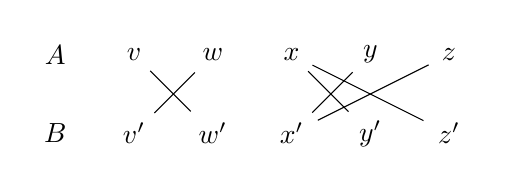
\begin{tikzpicture}
		\node[shape=circle] (A) at (-1,0) {$A$};
		\node[shape=circle] (v) at (0,0) {$v$};
		\node[shape=circle] (w) at (1,0) {$w$};
		\node[shape=circle] (x) at (2,0) {$x$};
		\node[shape=circle] (y) at (3,0) {$y$};
		\node[shape=circle] (z) at (4,0) {$z$};
		\node[shape=circle] (B) at (-1,-1) {$B$};
		\node[shape=circle] (v') at (0,-1) {$v'$};
		\node[shape=circle] (w') at (1,-1) {$w'$};
		\node[shape=circle] (x') at (2,-1) {$x'$};
		\node[shape=circle] (y') at (3,-1) {$y'$};
		\node[shape=circle] (z') at (4,-1) {$z'$};

		\path [-] (v) edge (w');
		\path [-] (x) edge (y');
		\path [-] (x) edge (z');
		\path [-] (v') edge (w);
		\path [-] (x') edge (y);
		\path [-] (x') edge (z);
	\end{tikzpicture}}}
	\caption{Example of how all graphs have a bipartite representation}
	\label{Figure 0}
\end{figure}

\par All graphs $G=(V,E)$ have a bipartite representation $G'=(A\cup B,E')$. Considering the example in \texttt{Figure 1}, defining $A=V$, $B$ to a be a copy of $V$, and the edge set \newline${E'=\{(u,v'):(u,v)\in E,u\in A,v'\in B\}}$ generates a bipartite presentation of $G$. The bipartite representation has twice the number of edges since each edge $(u,v)$ is now replaced by two edges $(u,v')$ and $(v,u')$. %TODO in practice we don't need these duplicates

\par The \textit{Neighbourhood} of a vertex $v$ is the set of vertices which share an edge with, $N_v=\{u:(u,v)\in E\}$. The \textit{Degree} of a vertex $v$ is the size of its neighbourhood, $\delta_v=|N_v|$. A vertex $v$ is \textit{$s$-sparse} if its degree is less than, or equal to, $s$.
\par The \textit{Edge Vector} of a vertex $v$ of length $|V|$ where each index gives the weight of the edge from $v$ to the vertex associated with that index. Typically a weight of 0 is stored if no edge exists between $v$ and a specific vertex. The graphs used in this project are unweighted so the values in the edge vector are booleans describing whether, or not, an edge exists. These edge vectors can be stored as bitstrings.
\par \textit{Graph Streams} are an unbounded sequence of instructions $\{e_1,e_2,\dots\}$ which describe how to construct the graph. These instructions $e_i$ describe modifications to the edges of a graph. The vertex set of the described graph is inferred from the instructions. In this project we are only concerned with two types of graph stream. %TODO something about the unbounded part??
\begin{itemize}
	\item \textit{Insertion-Only Streams} where each instruction inserts a new edge to the graph. It is assumed that no edges are inserted multiple times. For the unweighted, undirected graphs used in this project insertion-only streams are a list of the edges in the graph and can be read in any order. Here the instructions have the form $e_i=(u,v)$ where $u,v\in V$ are the endpoints of the edge being inserted.
	\item \textit{Insertion-Deletion Streams} where each instruction either adds a new edge to the graph or removes an existing edge from the graph. It is assumed that no edges are inserted multiple times, nor is an edge removed if it is not currently in the graph. For the unweighted, undirected graphs used in this project instructions of insertion-deletion streams take the form $e_i=(\Delta,u,v)$ where $u,v\in V$ are the endpoints of the edge and $\Delta$ is a boolean defining whether $e_i$ is an insertion or deletion instruction. The order of instructions is clearly important for insertion-deletion streams.
\end{itemize}
Other versions of graph streams exist which allow for changes to the weights of edges and directed edges, but these are out of scope for this project.

\par \textit{Streaming Algorithms} are algorithms which are designed to take a stream of sequential instructions as their input. Streaming algorithms are space-efficient since only one instruction is read at a time, requiring constant space. Streaming algorithms which only require a single pass of the instruction stream are called \textit{Online Algorithms}. Online algorithms have the advantage of being able to take new instructions without having to recompute anything.

\par An \textit{$\alpha$-Approximation Algorithm} is an algorithm which returns a result within an $\alpha$ factor to the optimal solution to the problem. Algorithms which solve the \texttt{Neighbourhood Detection Problem} are $\frac1c$-approximation algorithms since they only return $d/c$ of the neighbours of a vertex which we know to have at least $d$ neighbours.

\par A family of hash functions $\mathcal{H}=\{h:X\to Y\}$ is described as being \textit{Pairwise Independent} if $\forall\ u,v\in X$ with $u\neq v$ and $\forall\ a,b\in Y$ if $h$ is chosen uniformly at random from $\mathcal{H}$ then $\mathbb{P}(h(u)=a\wedge h(v)=b)=\frac1{|Y|^2}$. This means that the values $u,v$ are hashed to are assigned uniformly at random and pairwise independently.

\par A family of hash functions $\mathcal{H}=\{h:X\to Y\}$ is described as begin \textit{$k$-Wise Independent} if for any $k$ distinct elements of $X$ $\{v_1,\dots,v_k\}$ and any, not necessarily distinct, elements of $Y$ $\{a_1,\dots,a_k\}$ if $h$ is chosen uniformly at random from $\mathcal{H}$ then $$\mathbb{P}(h(v_1)=a_1\wedge\dots\wedge h(v_k)=a_k)=\frac1{|Y|^2}$$
\section{Technologies}
%\begin{itemize}
%	\item C++
%	\begin{itemize}
%		\item Low level
%		\item Memory manipulation
%		\item Faster
%		\item Perhaps something about why not java or python etc.
%	\end{itemize}
%	\item Standard library online
%\end{itemize}
For the implementations in this project I chose to use C++, specifically \texttt{C++11}. I initially considered using either python or C++, as they both work in the object-orientated paradigm and I am proficient in both. I chose C++ as it allows for more control with memory management and typically has faster run-times. For this project the memory management is more important as I am looking to evaluate the space-efficiency of algorithms. The faster run-times is important when evaluating the practicalities of the algorithms.
\par I limited myself to using the \textit{C++ Standard Library} \texttt{std} as the underlying implementations of this library are well document. This was particularly important for the abstract data types I used as I could check what the underlying implementations and adjust my evaluation accordingly. When implementing randomness I used the \texttt{<random>} module of \texttt{std} and seeded the generators with the current time so that each run would have a different generator.

\section{Evaluation Approach}

% TODO expectations
%\begin{itemize}
%	\item What features are tested (time \& space)? How?
%	\item Against naïve algorithm.
%	\item Insertion-Only v Insertion-Deletion algorithm for insertion-only streams.
%\end{itemize}

%TODO talk about verifying my results
%TODO typical test = vary c between [3,20]. set d=max degree

During evaluation three performance metrics were measured: success-rate, time-taken, and, space-used. These are all interconnected and come with their own trade-offs. Typically, the changes to space-used and time-taken when different strategies are implemented occur in the same direction, but at different rates. During most tests the success-rate was near perfect, but the other metrics were significantly higher as it took longer for a solution to be found.

\par In real world scenarios we are most interested analysing the neighbourhoods of the most influential vertices. For this reason $d$ is set to the maximum degree in the graph during all tests. Further, the greater the proportion of a neighbourhood returned the better the inferences made are so I focussed testing on low values of $c$, namely $c\in[1,20]$.

\par For this project I wanted some graphs generated from the real-world. I found a collection of large graph streams, from different applications, in the \texttt{Stanford Network Analysis Project} (\texttt{SNAP}) datasets collection \cite{SNAP}. I chose to use the graphs generated from social networks as I found that application most motivating, but this choice is essentially arbitrary. The graph streams from \cite{SNAP} were all insertion-only so I wrote a utility program which created insertion-deletion streams from them by using a Bernoulli random variable to decide whether to delete an edge immediately after inserting it. \textbf{Table 1} provides details about the graphs used during evaluation.

\begin{center}
	\begin{table}[h]
		\tiny
		\begin{tabular}{|l|l|l|l|l|l|l|l|}
			\hline
			\textbf{Name}&\textbf{Type}&\textbf{\# Vertices}&\textbf{\# Edges}&\textbf{\# Instructions}&\textbf{Max Degree}&\textbf{File Size}\\
			\hline
			$\mathtt{facebook\_small}$&Insertion-Only&52&146&-&18&3 KB\\
			$\mathtt{facebook\_small\_deletion}$&Insertion-Deletion&52&131&161&16&5 KB\\
			$\mathtt{facebook}$&Insertion-Only&747&30,025&-&293&587 KB\\
			$\mathtt{facebook\_deletion}$&Insertion-Deletion&747&26,718&33,332&267&846 KB\\
			$\mathtt{gplus}$&Insertion-Only&12,417&1,179,613&-&5,948&12 MB\\
			$\mathtt{gplus\_deletion}$&Insertion-Deletion&12,417&1,049,309&1,309,917&4,998&16 MB\\
			$\mathtt{gplus\_large}$&Insertion-Only&102,100&30,238,035&-&104,947&1.3 GB\\
			\hline
		\end{tabular}
    \caption{Details of graphs used during evaluation}
	\end{table}
\end{center}

\chapter{Insertion-Only Streams}

\section{Degree-Based Reservoir Sampling}

\texttt{Degree-Based Reservoir Sampling} is a technique for uniformly sampling a vertex from the set of vertices whose degrees are greater than a specified minimum bound $d_1$ along with $d_2$ of its neighbours. The sampler maintains a subset of the vertices of degree $d_1$, known as the \textit{reservoir} \cite{degResSampling}, and stores the first $d_2$ of the edges incident to a vertex after it is added to the reservoir. The size of this reservoir is a parameter of the algorithm. \textbf{Algorithm 1} outlines pseudocode for performing \texttt{Degree-Based Reservoir Sampling} on a bipartite graph using an insertion-only graph stream.

\begin{algorithm}[H]
	\caption{\texttt{Degree-Based Reservoir Sampling}$(d_1,d_2,s)$}
	\SetKwInOut{Require}{require}
	\Require{Degree bound $d_1\in\nats$, Neighbourhood bound $d_2\in\nats$, Reservoir size $s\in\nats$, Insertion-only stream $\{(a_0,b_0),\dots,(a_n,b_n)\}$}
	$D\leftarrow\{\}$ \tcp*{Degree counter}
	$R\leftarrow\{\}$ \tcp*{Reservoir}
	$E\leftarrow\{\}$ \tcp*{Collected edges}
	$x\leftarrow0$\tcp*{\# nodes of degree$\geq d_1$}
	\For{$i\in[0,n]$} {
		$D[a_i]\leftarrow D[a_i]+1$\tcp*{Increment degree counter}
		\If{$D[a_i]\equiv d_1$}{
			\tcp{Consider inserting $a_i$ to reservoir}
			$x\leftarrow x+1$\\
			\If{$|R|<s$} {
				\tcp{Reservoir is not full}
				$R\leftarrow R\cup\{a_i\}$
			} \Else {
				\tcp{Reservoir is full}
				\If{\texttt{Bernoulli}$\left(\frac{s}x\right)$} {
					Let $a'$ be a uniform random element of $R$\tcp*{Element to replace}
					Delete edges in $E$ incident to $a'$\\
					$R\leftarrow(R\backslash\{a'\})\cup\{a\}$\tcp*{Swap $a_i$ and $a'$}
				}
			}
		}
		\If{$a_i\in R$ \textbf{and} $D[a_i]< d_1+d_2$}{
			$E\leftarrow E\cup(a_i,b_i)$\tcp*{Store edge}
		}
	}
	\If{$\exists\ a\in R$ with $D[a]\geq d_1+d_2-1$} {
		\Return{Uniform random vertex and neighbourhood from those of size $d_2$}
	} \lElse { \Return{\texttt{FAIL}}}
\end{algorithm}

\par Three data stores are used in \texttt{Degree-Based Reservoir Sampling}: a \texttt{map} of the degree of every node in the graph $D$; a \texttt{set} for the reservoir $R$; and a \texttt{set} for edges incident to the vertices in the reservoir $E$.

\par The reservoir $R$ has an invariant that at any point in time it contains a uniform sample of the vertices whose degrees are known to be greater than $d_1$. This invariant is proved as \textbf{Lemma 2.1}, first I shall describe how the reservoir is maintained by controlling how vertices are inserted. The first time the degree counter for a vertex $v$ surpasses $d_1$, $v$ is considered for insertion into the \textit{reservoir}. There are two cases
\begin{itemize}
	\item If the reservoir is \underline{not} full (\ie $|R|<s$) then $v$ is inserted into the reservoir.
	\item Otherwise, a Bernoulli random variable with probability $p=\frac{x}s$ is used, where $x$ is the number of vertices known to have degree at least $d_1$. If this random variable succeeds then pick, uniformly at random, a vertex $u$ currently in the reservoir and replace it with $v$. All the edges in $E$ which are incident to $u$, and no other vertex in the reservoir, are removed from $E$.
\end{itemize}

Whenever an edge $(u,v)$ is encountered and $u$ is in the reservoir and the number of edges stored in $E$ incident to $u$ is less than $d_2$ then $(u,v)$ is inserted into $(u,v)$. %TODO rewrite this
\begin{adjustwidth}{.3cm}{}\fbox{\parbox{\textwidth}{

\textbf{Lemma 2.1} At time $t$, $R$ contains a uniform sample of the vertices whose degrees are known to be at least $d_1$.\\

\textit{Proof (by induction)}\\
Let $X_t$ be the set of vertices whose degrees are know to be greater than $d_1$ after $t$ instructions have been consumed and $x_t:=|X_t|$.\\
\underline{Base Case} - $x_t\leq s$.\\
Trivially true since $R$ is not yet full so $R=X_t$.\\
\underline{Inductive Case} - $x_t>s$.\\
Assume the property holds for $x_t=z>s$, then the probability of any given element of $X_t$ is in $R$ is $\frac1z$.
Without loss of generality, let $a$ be the next element considered for sampling and $b$ be any element of $R$. The probability $a$ is sampled is $\frac{s}{z+1}$ and, given $a$ is to be sampled, the probability $b$ is chosen for removal is $\frac1s$. Thus, the probability that $b$ is replaced by $a$ is $\frac{s}{z+1}\cdot\frac{1}{s}=\frac1{z+1}$. Similarly, the probability $b$ is \underline{not} replaced by $a$ is $1-\frac1{z+1}=\frac{z}{z+1}$. By the inductive hypothesis, the probability that $b$ was in $R$ was $\frac1z$. Thus, the probability that $b$ is still in $R$ is $\frac1z\times\frac{z}{z+1}=\frac1{z+1}$.\\

Hence by mathematical induction, $R$ contains a uniform sample of the vertices of sufficient degree at all points in time.$\hfill\square$
}}\end{adjustwidth}\vspace{.3cm}
%TODO adding termination condition? Maybe add during implementation

\par If $v$ is not added to the reservoir at this time, it never will be in the future. Note that in the case that the reservoir is full and $v$ is inserted into it, $v$ is replacing an element that was in the reservoir meaning any progress made towards finding a neighbourhood for that vertex is annulled. The amount of progress is not taken into account and thus if there is a high turn-over of elements in a reservoir then less progress is made towards finding a neighbourhood for each of them. This is discussed further during evaluation.

\par \texttt{Degree-Based Reservoir Sampling} only works on insertion-only streams as it does not account for when the degree of a vertex falls below the threshold, after being sampled. This means the reservoir may contain vertices whose degree is less than $d_1$.

\par For this project we are interested in how \texttt{Degree-Based Reservoir Sampling} can be implemented for bipartite graphs, specifically we want to sample from the $A$-vertices of the graph. For a bi-partite graph with $n$ $A$-vertices \texttt{Degree-Based Reservoir Sampling} requires $\mathcal{O}(n\log n+sd_2\log n)$ space, assuming $O(\log n)$ space is required to store an edge or a vertex, since it stores a degree counter for every $A$-vertex and at most $d_2$ edges for each of the $s$ vertices in the reservoir.

\section{Proposed Algorithm}

%\begin{itemize}
%	\item Assumptions: no duplicate edges (can mitigate cases when this would be required by being smart)
%	\item Insertion stream neighbourhoods cannot be diminished over time.
%	\item Possibility of failure (missed edges) \& mitigation
%	\begin{itemize}
%		\item Theorem 3.2 (probs not proof)
%	\end{itemize}
%	\item Theoretical space requirements
%\end{itemize}

\texttt{Neighbourhood Detection} can be solved using \texttt{degree-based reservoir sampling} by setting $d_2=\frac{d}c$. The question remains as to what to set $d_1$ and $s$ to in order to achieve a high probability of success. \textbf{Algorithm 2} is the space-efficient algorithm proposed in \cite{orig} for solving \texttt{Neighbourhood-Detection} for insertion-only streams.

\begin{algorithm}
	\caption{One-pass $c$-Approximation Insertion-Only Streaming Algorithm for $\mathtt{Neighbourhood\ Detection}$}
	\SetKwInOut{Require}{require}
	\Require{Space $s$, degree bound $d$.}
	$s\leftarrow\lceil\log(n)\cdot n^{\frac1c}\rceil$\\
	\For{$i\in[0,c-1]$\text{\textbf{ in parallel}}} {
		$(a_i,S_i)\leftarrow\mathtt{Deg}\mbox{-}\mathtt{Res}\mbox{-}\mathtt{Sampling}\left(\max\left\{1,i\cdot\frac{d}{c}\right\},\frac{d}c,s\right)$
	}
	\Return{\small Uniform random neighbourhood $(a_i,S_i)$ \text{from successful runs}}
\end{algorithm}

\par In \cite{orig} it is proven that setting $s=\left\lceil\ln(n)\cdot n^{\frac1c}\right\rceil$ and using $c$ \texttt{degree-based reservoir samplers} each with a different lower bound, incremented from $\frac{d}c$ to $d$ stepping by $\frac{d}c$ each time, results in a high probability of success. The samplers are run in parallel so that the algorithm only requires a single pass of the stream. Implementing parallel running of the samplers just requires passing the same instruction to each sample before fetching the next instruction.

\par Each of the $c$ samplers requires $\mathcal{O}(n\log n+sd_2\log n)$ space. Since the degree map can be shared between samplers the total space is $\mathcal{O}(n\log n+c\cdot sd_2\log n)=\mathcal{O}(n\log n+n^{\frac1c}d\log^2n)$. The proposed algorithm does require you to know the number of vertices in the graph stream before running the algorithm, or at least the $\log$ of it. If this is unknown then it is quick to run through the whole stream and build a set of vertices in the graph. This requires $\mathcal{O}(n\log n)$ space, assuming $O(\log n)$ space is required to store a vertex. However, in many real-world scenarios this number (or a good approximation) will be known due to it being important for other tasks.

\section{Implementation}

\par The graphs from \cite{SNAP} are not formatted in a strictly bipartite way. I adjusted \texttt{degree-based reservoir sampling} to account for this by repeating \texttt{lines 6-17} (and the early termination clause) of \textbf{Algorithm 1} after the end of the \texttt{for} loop, with all occurrences of $a_i$ replaced by $b_i$.

\begin{figure}[H]
	\label{Figure 2}
	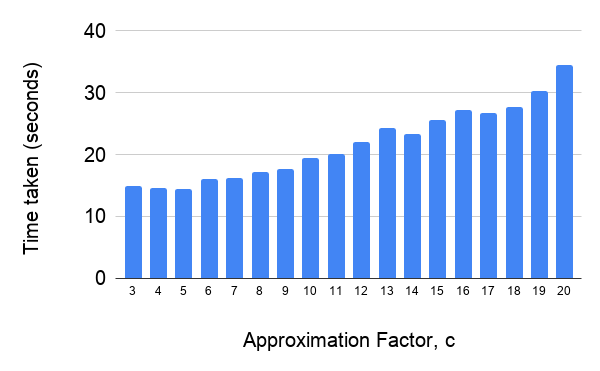
\includegraphics[width=.5\textwidth]{img/gplusInitialTime.png}
	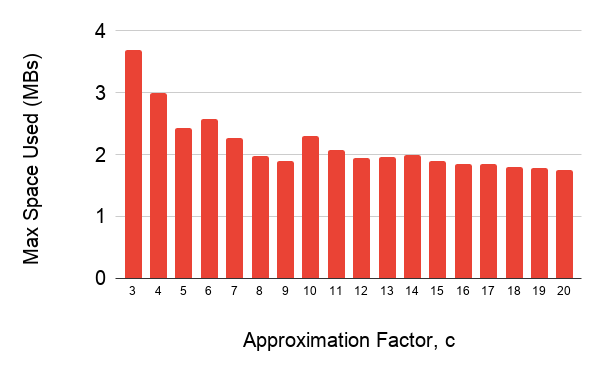
\includegraphics[width=.5\textwidth]{img/gplusInitialSpace.png}
	\caption{Results from testing initial implementation of \textbf{Algorithm 2} on \texttt{gplus} graph for different approximation factors}
	%"Final Evaluation - insertion-only"/Master
\end{figure}

\par During this section I tested changes to the implementation on multiple graphs, for brevity and succinctness I shall only show the results for \texttt{gplus}. \texttt{Figure 2.3.1} shows the results of testing the initial implementation of \textbf{Algorithm 2}. These results shows that the space requirements of \textbf{Algorithm 2} are significantly less than the size of file stream and that the space requirements decrease as the approximation factor increases but there is an undesirable result that the time taken increases as the approximation factor increases.

\par After this initial implementation I considered two alterations to the implementation:
\begin{enumerate}
	\item \textit{Early Termination} - Returning the first neighbourhood of sufficient size, rather than uniformly sample from all which succeed; and,
	\item \textit{Shared Edge-Set} - Having all samplers share an edge-set, rather than each have one each.
\end{enumerate}

\subsection{Early Termination}

\textbf{Algorithm 1} states that the whole stream should be run through before the sampler returns a result uniformly from those which succeeded. This is unnecessary to fulfil \texttt{neighbourhood detection} as returning the first successful result would be sufficient. Similarly \textbf{Algorithm 2} states that all samplers should be run to completion and then a result is returned from those which succeeded. Again, this is unnecessary as return the first encountered neighbourhood of sufficient size would suffice for solving \texttt{neighbourhood detection}. These early terminations can be implemented by terminating the algorithm after it finds a vertex of degree $d_1+d_2-1$ which is in a reservoir (remembering that $d_1$ is different for each reservoir).

\par Implementing early termination should reduce run-time as only part of the stream is being consumed and should reduce space used by the edge-sets in reservoir sampling as no data is stored after the first solution is found. As this change terminates at the first success there is no change to the success rate of the algorithm. One down side is that you will likely get less variety in the returned neighbourhoods as the algorithm will not encounter every vertex which meets the degree requirements, however this is not relevant to the problem.

\begin{figure}[H]
	\label{Figure 3}
	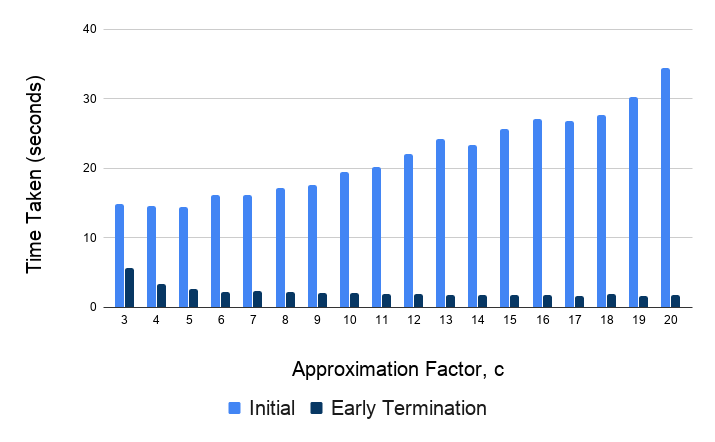
\includegraphics[width=.5\textwidth]{img/gplusEarlyTerminationTime.png}
	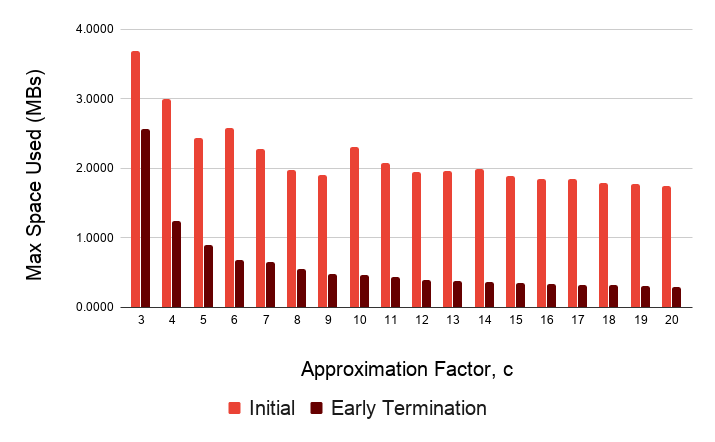
\includegraphics[width=.5\textwidth]{img/gplusEarlyTerminationSpace.png}
	\caption{Results when using early termination, tested on \texttt{gplus} graph for different approximation factors. Against the results for the initial implementation.}
	%"Final Evaluation - insertion-only"/Master
\end{figure}

\par \texttt{Figure 2.3.2} shows the results implementing early termination, against not implementing it, for graph \texttt{gplus} at different approximation factors. The time taken now decreases as $c$ increases and is more than halved in all cases. The space-requirements are down in every case and are down more than $90\%$ for reasonable values of $c$. Both metrics now converge quickly, to $\smallsim\!\!1.5$ seconds and $3.3$MBs respectively, meaning we can make predictions on the performance of the algorithm for greater values of $c$. These are really good results, so I implemented this change going forward. %TODO explain reasons behind these results
%NOTE space converged to is that used by degree map
%TODO comment about effect on space used by reservoirs vs degree map
%TODO this change means that time taken is now a measure of success as failure is (basically) the only time the whole stream is run through

\subsection{Shared Edge-Set}

\vspace{.3cm}\begin{adjustwidth}{.3cm}{}\fbox{\parbox{\textwidth}{

\textbf{Lemma 2.2} If \textbf{Algorithm 2} terminates after the first sufficient neighbourhood it finds, no vertex occurs in multiple reservoirs at the same time.\\

% TODO a proof by contradiction
\textit{Proof (by contradiction)} Let $v$ be a vertex in the graph stream. Suppose, without loss of generality, that $v$ is a member of the reservoirs of both \texttt{Deg-Res-Sampling}$(\frac{d}{c},\frac{d}{c},s)$ and \texttt{Deg-Res-Sampling}$(\frac{2d}{c},\frac{d}{c},s)$. This means that $v$ was sampled twice, after encountering the $\frac{d}c^\text{th}$ \underline{and} $\frac{2d}c^\text{th}$ edge incident to $v$ in the stream. After sampling $v$ for the first time, encountered edges which are incident to $v$ are stored. This means that by the time $v$ is sampled for the second time $\frac{2d}c-\frac{d}c=\frac{d}c$ edges incident to $v$ have been stored. This is a sufficient neighbourhood for \textbf{Algorithm 2} to terminate. This is a contradiction since termination occurs before the second sampling occurs.$\hfill\square$

}}\end{adjustwidth}\vspace{.3cm} %TODO refine

\par A consequence of \textbf{Lemma 2.2} is that an edge is only stored in multiple edge sets if its endpoints are sampled by different samplers. %TODO mention this is rare
This means that introducing a shared edge-set for all samplers will have little effect on the space requirements of \texttt{Algorithm 2}.
\par However, the alterations to the implementation, which would have to made to allow for a shared edge-set, could introduce time savings. Namely, a data-structure is required to store \underline{precisely} which reservoir each vertex is in so that the appropriate value of $d_1$ is used in \texttt{Algorithm 1:Line 18}, otherwise improper termination could occur. An appropriate data-structure for this would be a \texttt{map} from each vertex to a bitstring whose indices indicate whether the vertex lies in an associated reservoir. With this implementation, inserting or deleting a vertex to/from a reservoir and querying whether a vertex is in a given reservoir is achieved with a single query of a \texttt{map} and then a known bit in a bitstring which both take $\mathcal{O}(1)$ time. This \texttt{map} replaces the \texttt{ordered set}s currently used to store the reservoirs of each sampler and thus reduces these action times from $O(\log n)$ to $\mathcal{O}(1)$ time. As these actions occur a lot this change should result in a reasonable reduction in run-time. % TODO something about space used to store a vertex in the map vs in sets

\begin{figure}[H]
	\label{Figure 4}
	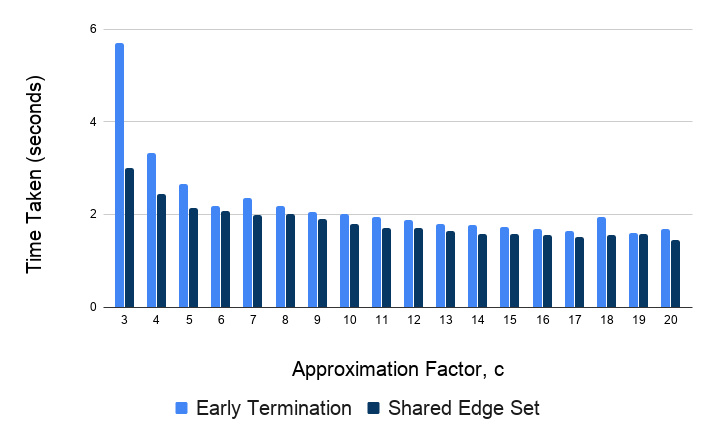
\includegraphics[width=.5\textwidth]{img/gplusSharedEdgeSetTime.png}
	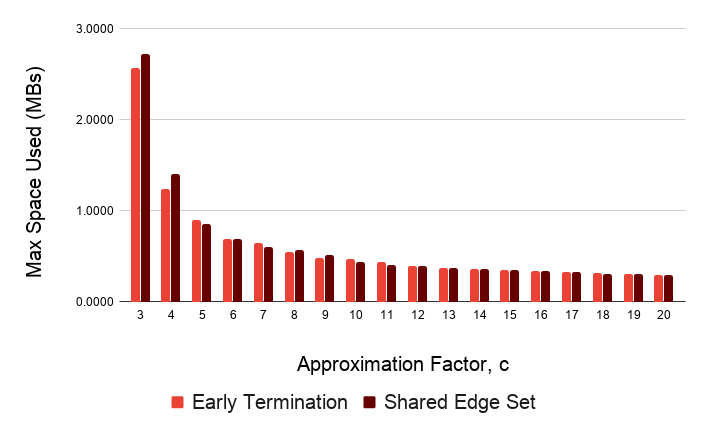
\includegraphics[width=.5\textwidth]{img/gplusSharedEdgeSetSpace.png}
	\caption{Results when using early termination and a shared edge set, tested on \texttt{gplus} graph for different approximation factors. Against the results just using early termination.}
	%"Final Evaluation - insertion-only"/Master
\end{figure}

\par \texttt{Figure 2.3.3} shows the results when implementing both early termination and a shared edge set, against only using early terminiation. These tests showed a consistent reduction in run-time when both strategies are used. there is a slight increase in space usage for low values of $c$ but this difference disappears very quickly so is of little concern. Implementing a shared-edge set does not change the logic of the algorithm so does not affect its success rate. Due to the reduction in mean run-time and no noteworthy changes in space requirements, I recommend implementing this change.

%TODO discuss performance against theory
\section{Parameter Tuning}

%\begin{itemize}
%	\item Vary size of reservoir ($s$) \& number of samplers together to find an optimum
%	\item Full optimised against v Naïve.
%\end{itemize}

\par The changes discussed in \textbf{Section 2.4} have been to the technical implementation of \textbf{Algorithm 2}, rather than to the its logic. This means these changes have had no affect on the success rate of the algorithm. I will now discuss potential changes to the logic of the proposed algorithm. These changes will affect the success rate of the algorithm. As I am investigating the practicalities of the algorithm keeping the run-times usable is a high priority. In \textbf{Algorithm 2} there are two parameters to scrutinise: the number of samplers; and, the size of the reservoirs $s$.

\par The total reservoir size, $\left\lceil\ln(n)n^{\frac1c}\right\rceil\times\text{\#\ Samplers}$, is the main factor affecting the space-used by the algorithm as this is the number of vertices it needs to store edges for. Noting that \textbf{Algorithm 2} sets the number of samplers to be $c$ and that $cp\left\lceil\ln(n)n^{\frac1c}\right\rceil\leq c\left\lceil p\ln(n)n^{\frac1c}\right\rceil\ \forall\ p\in[0,1]$ it is apparent that reducing the number of samplers has a greater effect on total reservoir size, and thus space-used, than reducing reservoir size by the same proportion. For this reason I investigated the number of samplers first.

\subsection{Number of Samplers}

\par When changing the number of samplers we need to consider their lower bounds $d_1$ too. If the range of vertex degrees $[d_1,d_1+d_2]$ which individual samplers sample at overlap then duplicate sampling of vertices can occur which offers no advantages and leads to a reservoir space being wasted. And, if there are gaps between these ranges then there are vertices which may not be sampled. %TODO flesh this out more.
Thus, the best set up is to have the sampling ranges be sequential with no gaps and so when varying the number of samplers we should only add or remove from the endpoints of these ranges.

\par The samplers with lower lower-bounds $d_1$ start sampling earlier and from a larger pool. I expect these early samplers to be more important wrt performance gains, than later samplers. It is not necessarily true that the first sampler is the most important as it is sampling from the largest pool and so has the greatest turn-over rate in its reservoir.

\begin{figure}[H]
	\label{Figure 5}
	\subfloat[Removing early samplers]{{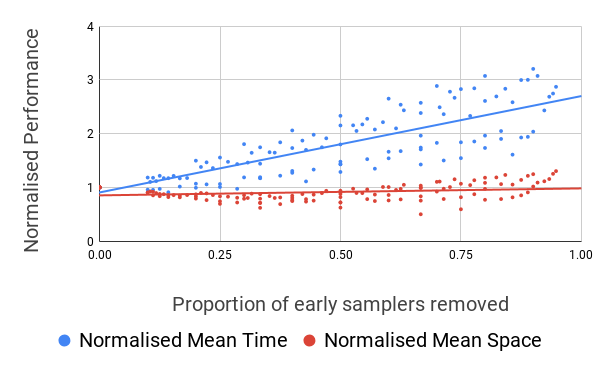
\includegraphics[width=.5\textwidth]{img/gplusRemoveEarly.png}}}
	\subfloat[Removing late samplers]{{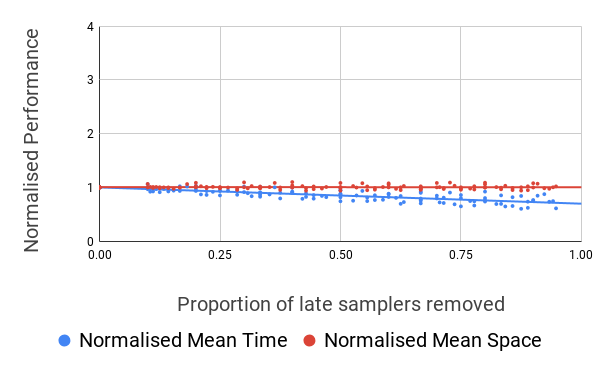
\includegraphics[width=.5\textwidth]{img/gplusRemoveLate.png}}}
	\caption{Results when removing different proportions of samplers, either from the start or end of the sampler range, for different values of $c$. These results are normalised with the values when no samplers are removed being 1 for that value of $c$. Results from graph \texttt{gplus}.}
	%"Final Evaluation - insertion-only"/Master
\end{figure}

\par Two tests where run to investigate what had a greater effect on performance, removing later samplers or earlier samplers.
\begin{enumerate}
	\item Removing the \underline{first} $x$ samplers from \texttt{Algorithm 2} for $x\in[1,c)$, for $c\in[1,20]$.\\
	\textit{i.e.} Change the \texttt{for} loop in \texttt{Algorithm 2:Line 2} to run for $i\in[x,c-1]$.
	\item Removing the \underline{last} $x$ samplers from \texttt{Algorithm 2} for $x\in[1,c)$, for $c\in[1,20]$.\\
	\textit{i.e.} Change the \texttt{for} loop in \texttt{Algorithm 2:Line 2} to run for $i\in[0,c-x]$.
\end{enumerate}

\par \texttt{Figure 2.4.4} shows the results of these tests, with the results normalised to make them comparable. These results confirm the hypothesis that the lower a sampler's lower-bound is, the greater the effect of its inclusion on performance. Time-taken increased as more early samplers were removed, and decreased as more late samplers were removed. The space used was not affected much by the removal of samplers, although there is a slight increase in space usage when more early samplers were removed. Comparing the normalised results shows that removing early samplers is more detrimental to performance than including late samplers. This is due to late samplers only starting to sample later and they may not have begun sampling by the time one of the previous samplers has succeed, terminating the algorithm. When the same proportion of samplers were removed for different values of the  $c$, the relative performance was worse for greater values of $c$. This is to be expected as the real number of samplers removed increases with $c$.

\begin{figure}[H]
	\label{Figure 6}
	\centering
	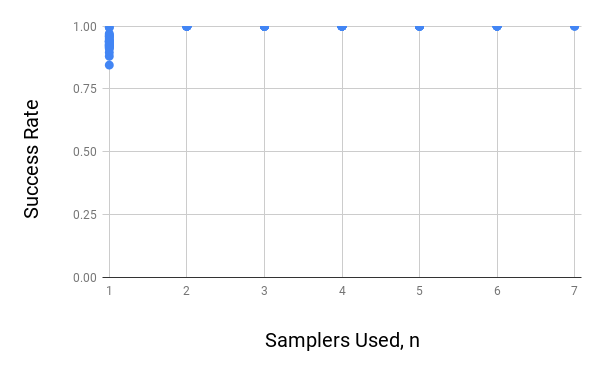
\includegraphics[width=.5\textwidth]{img/gplusSuccessRate.png}
	\caption{Success rate when only the first $n$ samplers are run on \texttt{gplus}.}
	%"Final Evaluation - insertion-only"/Master
\end{figure}

\par From these tests it is apparent that there are advantages to be found by removing late samplers, but not from removing the earliest. These tests did show that the failure rate does increase when too few of the early samplers are used. Thus I repeated the tests, this time testing using the first $n$ samplers for different values of $c$. \texttt{Figure 2.4.5} shows the results of this test and shows that the success rate dropped below 1 in the case that only the first sampler was used, in all other cases it was 1.

\par Running the first two samplers provided the best results. However, the largest graph I tested on only contains $~100,000$ vertices so this may not hold for significantly larger graphs. I suggest using the first $\mathtt{max}\left(2,\left\lceil\frac15\ln n\right\rceil\right)$ samplers. As we don't want the sampling ranges to overlap we need to add a restriction that the number of samplers is never greater than the approximation factor, giving the number of samplers used as $\mathtt{min}\left(c,\mathtt{max}\left(2,\left\lceil\frac15\ln n\right\rceil\right)\right)$.

\begin{figure}[H]
	\label{Figure 7}
	\subfloat[Time Taken]{{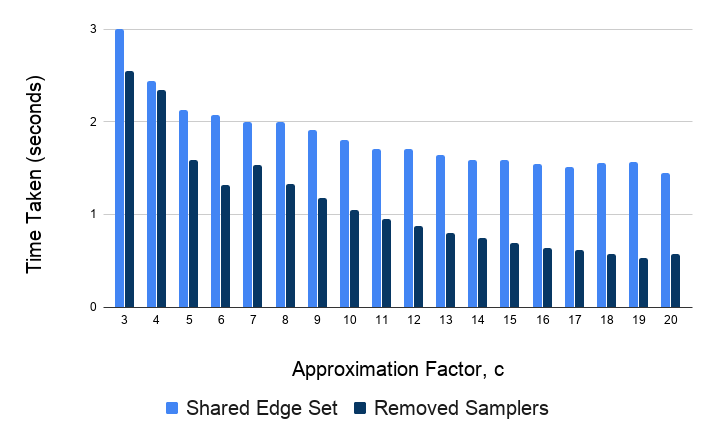
\includegraphics[width=.5\textwidth]{img/gplusRemovedSamplersTime.png}}}
	\subfloat[Space Used]{{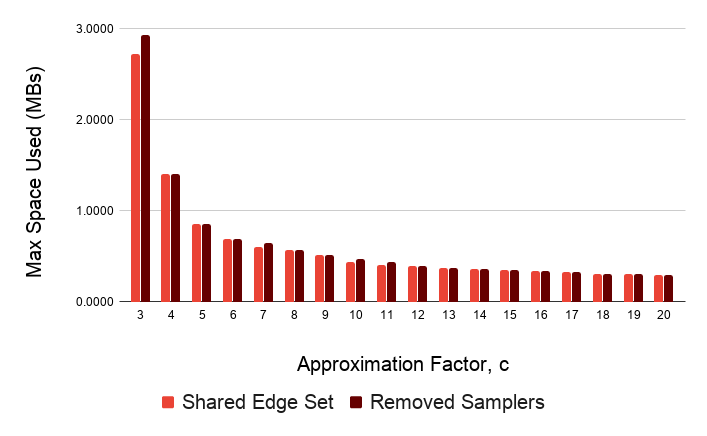
\includegraphics[width=.5\textwidth]{img/gplusRemovedSamplersSpace.png}}}
	\caption{Results when using a reduced number of samplers for different approximation factors, against just using the technical improvements. Results from graph \texttt{gplus}}
	%"Final Evaluation - insertion-only"/Master
\end{figure}

\par \texttt{Figure 2.4.6} shows the results when using the first $\mathtt{min}\left(c,\mathtt{max}\left(2,\left\lceil\frac15\ln n\right\rceil\right)\right)$ samplers against just using the technical improvements discussed in \texttt{Section 2.3}. As seen in \texttt{Figure 2.4.4}, the space usage is unchanged while the time taken is down in all cases. Run time is reduced by over $50\%$ for $c\geq 12$ and is below 1 second for larger values of $c$. A perfect success rate was maintained throughout these tests. Due to these good results, I implemented this change.
%TODO something about how the fact that space hasn't changed much means later samplers weren't coming into play often & thus sample size is unlikely to be important.
%TODO comment of special cases
\subsection{Reservoir Size}

\par \texttt{Figure 2.4.4 (b)} showed that removing late samplers had little effect on the space used by the algorithm. This is due to these samplers not getting the chance to sample very often as the algorithm often terminated before many vertices of sufficient degree were encountered. This means that reducing the size of those samplers would have had virtually no affect on the performance of the algorithm. This helps justify optimising the number of samplers before the sample sizes. The previous optimisation means that very few samplers are being run so it is unlikely that any great improvements will be found, if any, when reducing reservoir size.

\par Decreasing the reservoir size $s$ means less edges are stored, reducing space requirements, but increases the turn-over rate of the elements in the reservoir as the probability a vertex is sampled is the same but the reservoir size is smaller. The greater turn-over rate is detrimental to the success of the algorithm as it more likely for a vertex to be removed when it is close to succeeding. For very low sample sizes it is likely that the success rate of the algorithm will remain high, but the run-times will be dramatically increased.

\begin{figure}[H]
	\label{Figure 8}
	\subfloat[Time Taken]{{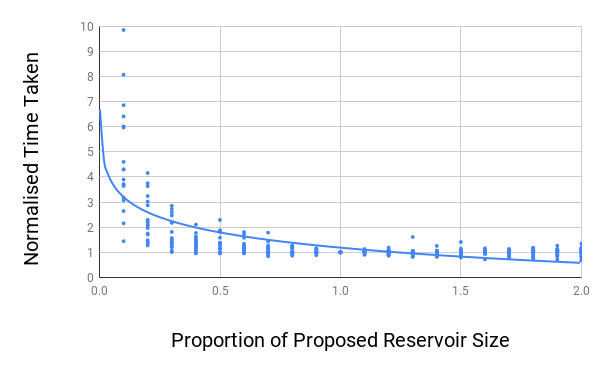
\includegraphics[width=.5\textwidth]{img/gplusReservoirSizeTime.png}}}
	\subfloat[Space Used]{{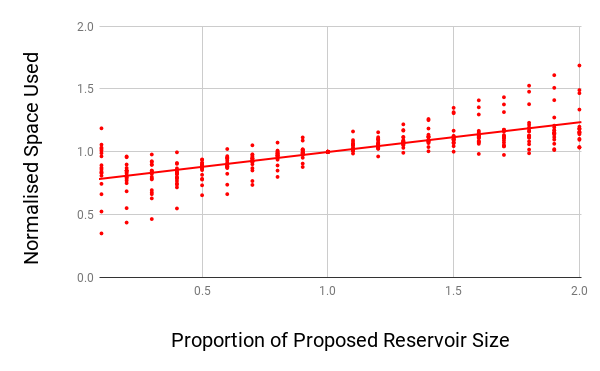
\includegraphics[width=.5\textwidth]{img/gplusReservoirSizeSpace.png}}}
	\caption{Normalised results when varying the reservoir size used on \texttt{gplus} for different approximation values. Results normalised by the result when the proposed reservoir size was used for each approximation valuee. (Using changes from \texttt{Section 2.3} and a reduced number of samplers)}
	%"Final Evaluation - insertion-only"/Master
\end{figure}

\par \texttt{Figure 2.4.7} shows the results when varying the reservoir size between $10\%$ and $200\%$ of the proposed size, for different values of $c$. The results are normalised to make them comparable across values of $c$. There is a positive linear relationship between space usage and reservoir size. The only inference that could be drawn from sample-size and time-taken is that there is a point at which time-taken dramatically increases, this is the point where the algorithm fails to find a sufficient neighbourhood. Overall, there is no clear strategy to improving the algorithm by varying the reservoir size.

%TODO mention theoretical space efficieny of this (should be same as before)
\par \textbf{Algorithm 3} gives \textbf{Algorithm 2} rewritten to include the proposed parameter optimisations.
\begin{algorithm}
	\caption{One-pass $c$-Approximation Insertion-Only Streaming Algorithm for $\mathtt{Neighbourhood\ Detection}$}
	\SetKwInOut{Require}{require}
	\Require{Space $s$, degree bound $d$.}
	$s\leftarrow\lceil\log(n)\cdot n^{\frac1c}\rceil$\\
	$n_s\leftarrow\min\left(c,\max\left(2,\left\lceil\frac15\ln(n)\right\rceil\right)\right)$\\
	\For{$i\in[0,n_s]$\text{\textbf{ in parallel}}} {
		$(a_i,S_i)\leftarrow\mathtt{Deg}\mbox{-}\mathtt{Res}\mbox{-}\mathtt{Sampling}\left(\max\left\{1,i\cdot\frac{d}{c}\right\},\frac{d}c,s\right)$
	}
	\Return{\small First neighbourhood of sufficient degree and its root}
\end{algorithm}

%TODO rewrite algorithm 2 with these parameter optimisations
\section{Evaluation}

%Run the following instances on different graphs \& compare
%\begin{itemize}
%	\item Initial implementation (no tuning, not quit early, not sharing)
%	\item Implementation with early quitting & shared edges
%	\item Implementation with tuned algorithm parameters
%	\item Naïve Implementation
%\end{itemize}
% Compare max space to size of edges file
% Identify which change had what effect (to space, time, success)

\begin{algorithm}
	\caption{Na\"ive Single-Pass Insertion-Only Streaming Algorithm for Neighbourhood Detection}
	\SetKwInOut{Require}{require}
	\Require{Stream $\{(s_0,t_0)\dots(s_n,t_n)\}$, degree bound $d$, precision bound $c$}
	$N\leftarrow\{\{\}\}\ \{\text{neighbourhoods}\}$\\
	\For{$i=0\dots n$} {
		append $t_i$ to $N[s_i]$\tcp*{Insert neighbour}
		\If{\text{size}($N[s_i])\geq d$} {
			\tcp{Sufficiently large neighbourhood found}
			$S\leftarrow \{N[s_i][0],\dots,N[s_i][\frac{d}{c}]\}$\tcp*{First $\frac{d}c$ elements of neighbourhood}
			\Return{($s_i,S$)}
		}
	}
	\Return{FAIL}\tcp*{No neighbourhoods found}
\end{algorithm}

\textbf{Algorithm 4} is a naïve algorithm for solving \texttt{neighbourhood detection} for insertion-only graph streams. This approach records the neighbourhood of every encountered vertex and returns the first one which surpasses the $\frac{d}c$ threshold. This algorithm will always succeed as there is a requirement that at least one vertex in the graph is of degree, at least, $d$. As the naïve algorithm terminates at the first neighbourhood of sufficient size and uses all edges in the stream up to that point, it is guaranteed to find the first vertex with a sufficient neighbourhood. This means the naïve algorithm is very quick, provided its space-usage is within the memory allocated to the algorithm. In the worst case, where all elements have degree $\frac{d}c-1$ except for the last which has degree $\frac{d}c$, $\frac{d}{c}+(n-1)(\frac{d}c-1)\in \mathcal{O}(n\frac{d}c)$ space is required. The average case has the same complexity and the best case, where the first $\frac{d}c$ instructions are incident to the same vertex, has $O(\frac{d}c)$ space-complexity.

To evaluate my final implementation I compared its performance to that of different stages of the optimisation and to the naïve implementation given in \textbf{Algorithm 4}. These different stages were
\begin{enumerate}[label=\roman*)]
	\item Initial Implementation - No early termination, shared edge-set or sampler removal. %insertionStreamsNotQuitEarly
	\item After Technical Optimisation - Implements early termination and a shared edge-set. %insertionStreamsSharedEdgeSet
	\item After Algorithmic Optimisation - Implements early termination, shared edge-set and sampler removal. %insertionStreamsRemovedSamplers
\end{enumerate}

\begin{figure}[H]
	\label{Figure 12}
	\subfloat[\texttt{gplus} - Time Taken]{{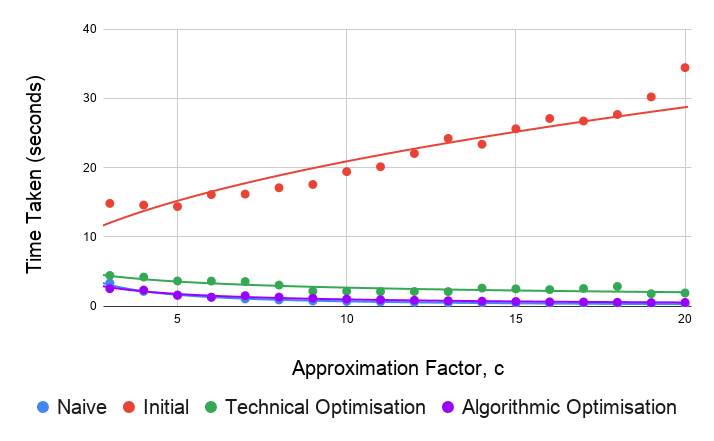
\includegraphics[width=.5\textwidth]{img/insertionOnlyGplusTime.png}}}
	\subfloat[\texttt{gplus} - Space Used]{{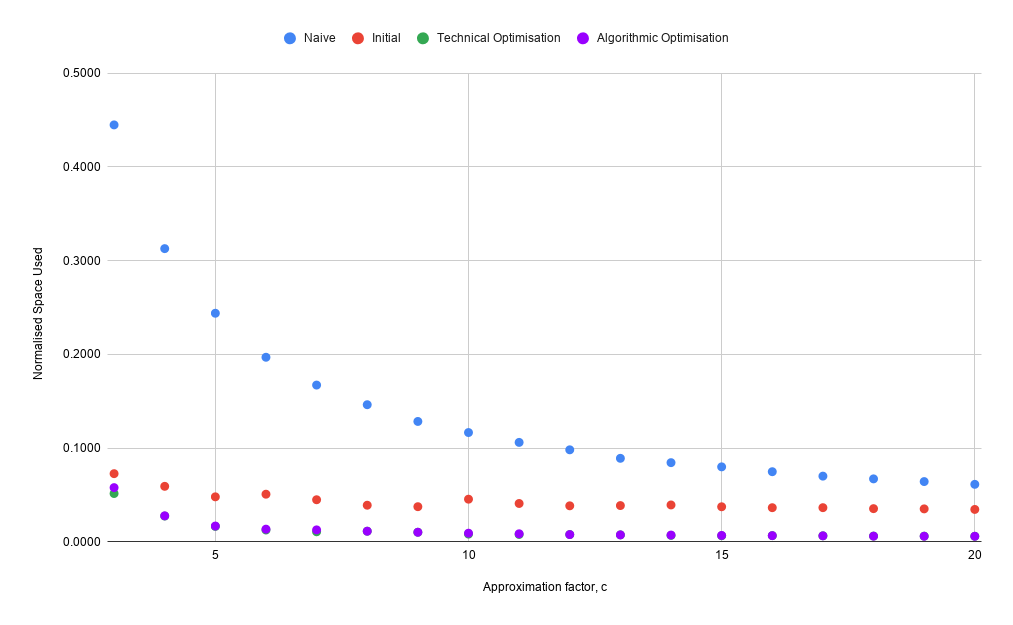
\includegraphics[width=.5\textwidth]{img/insertionOnlyGplusSpace.png}}}\newline
  \subfloat[\texttt{gplus\_large} - Time Taken]{{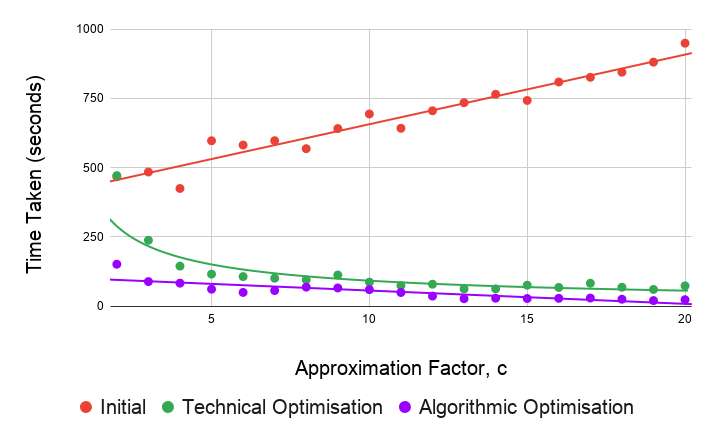
\includegraphics[width=.5\textwidth]{img/insertionOnlyGplusLargeTime.png}}}
	\subfloat[\texttt{gplus\_large} - Space Used]{{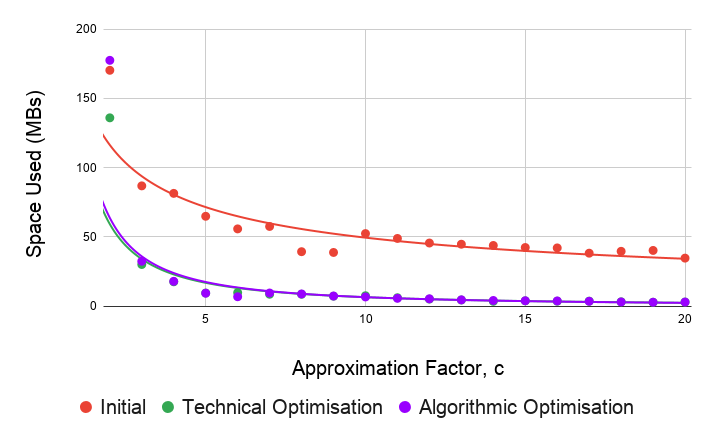
\includegraphics[width=.5\textwidth]{img/insertionOnlyGplusLargeSpace.png}}}
	\caption{Time taken and space used by different implementations of the proposed algorithm for insertion-only streams.}
	%"Final Evaluation - insertion-only"/Master
\end{figure}

\par \texttt{Figure 2.5.8} shows that the space usage was greatest for the naïve algorithm and lowest for the final implementation. The shortest run times came from the naive algorithm, followed by the final implementation. However, after three hours of computation the naïve algorithm had failed to return a result for the largest graph \texttt{gplus\_large} due to its high space usage. For the largest graph tested, \texttt{gplus\_large}, $13.7\%$ of the stream file size was required to find a 2-approximation using the initial implementation and only $1.39\%$ using the final implementation. This is a notable decrease in space requirements, meaning the algorithm can run efficiently on even large graphs.

\par The run time of the final implementation is useably quick: when run on \texttt{gplus\_large} it took $\sim\!\!150$ seconds to find a solution when $c=2$ and less than a minute for $c\geq5$. The naïve algorithm being quicker is irrelevant for this evaluation as it fails to terminate for larger files due to its space inefficiency.

\chapter{Insertion-Deletion Streams}

\section{$L_0$ Sampling}

%\begin{itemize}
%	\item L0 sampling uniformly samples from the non zero elements of a vector.
%	\item Break down into 1-sparse \& $s$-sparse recovery. (COMMENT ON SPACE USAGE)
%	\begin{enumerate}
%		\item Perfect $1$-sparse recovery uses a series of counters to determine whether a vector is exactly 1-sparse (ie exactly one non-zero element). If it is then it returns value of that index.
%		\item Give proofs that it works?
%		\item NOTE - if vector could have negative elements then other checks are require (in this usage they do not so don't worry)
%	\end{enumerate}
%	\begin{enumerate}
%		\item $s$-sparse uses pairwise hash function (explain these (maybe in preliminaries)).
%		\item $s$-sparse recovers an $s$-sparse (ie upto $s$ non-zero indices) vector of the passed vector.
%		\item Each index is considered by $r$ 1-sparse samplers.
%		\item NOTE $s$-sparse recovery space grows with $s$ so we want to use a small value (idea used during $L_0$ sampling)
%	\end{enumerate}
%	\item The formally proposed algorithm.
%	\item In this setting we consider the edge vector of each vertex (indicates which vertices it shares an edge with).
%\end{itemize}

%TODO citations
\par\texttt{$L_0$ Sampling} is a technique for sampling, approximately uniformly, from the non-zero indices of a vector when given a stream of updates to the weights of the indices. Here I shall describe one space-efficient technique for \texttt{$L_0$ Sampling} which succeeds with probability $1-\delta$ and requires $\mathcal{O}\left(\frac1\delta\log(1/\delta\gamma)\log^2(n)\right)$ space, this is significantly less than the $\mathcal{O}(n)$ space required to store the whole vector. This technique relies on two subroutines: \texttt{Perfect 1-Sparse Recovery}; and \texttt{Exact $s$-Sparse Recovery}. %TODO check space requirements (do I need to mention the two different success rates)

\subsection{Perfect 1-Sparse Recovery}

\par \texttt{Perfect 1-Sparse Recovery} takes a stream of updates and if the described vector is exactly $1$-sparse then it returns the index of the non-zero element, otherwise the routine fails. \textbf{Algorithm 5} provides an implementation \texttt{Perfect 1-Sparse Recovery} which works in cases where the weight of the non-zero element is non-negative. The non-negativity constraint is acceptable in this project as the graphs used as undirected and unweighted.

\begin{algorithm}
	\caption{\texttt{Perfect $1$-Sparse Recovery}}
	\SetKwInOut{Require}{require}
	\Require{Update Stream $\{(i,\Delta)\}$}
	$\phi,\iota,\tau\leftarrow0$\\
	\For{\textbf{all} updates $(i,\Delta)$} {
		$\phi\leftarrow\phi+\Delta$.\\
		$\iota\leftarrow\iota+i\cdot\Delta$.\\
		$\tau\leftarrow\tau+i^2\cdot\Delta$.\\
	}
	\If{$\iota^2\equiv\phi\cdot\tau$}{
		\tcp{Vector is $1$-Sparse}
		\Return{$\frac\iota\phi$}
		\tcp*{Index of non-zero entry}
	}\Else{
		\tcp{Vector is \underline{not} $1$-Sparse}
		\Return{\texttt{FAIL}}
	}
\end{algorithm}

\textbf{Algorithm 5} uses three counters: sum of the weights $\phi=\sum\Delta$; sum of the weights weighted by their index $\iota=\sum i\cdot\Delta$; and, the sum of the weights weighted by the their index squared $\tau=\sum i^2\cdot\Delta$. \textbf{Lemma 3.1} proves that $\iota^2\equiv\phi\cdot\tau$ is a sufficient test for whether the described vector is exactly $1$-sparse. If the vector is exactly $1$-sparse then $\iota/\phi$ is the index of the non-zero element and $\phi$ is its value. The only data stores are three counters each requiring $\mathcal{O}(\log n)$ space, thus \texttt{Perfect 1-Sparse Recovery} requires $\mathcal{O}(\log n)$ total space.

\vspace{.3cm}\begin{adjustwidth}{.3cm}{}\fbox{\parbox{\textwidth}{

\textbf{Lemma 3.1} $\iota^2\equiv\phi\cdot\tau$ \underline{iff} a vector is exactly $1$-sparse.\\

% TODO a proof by contradiction
\textit{Proof} Consider a vector where $i$ is the only non-zero index and that index stores value $u$.\\
Then $\phi=u,\ \iota=i\cdot u$ and $\tau=i^2\cdot u$. This means
$$\iota^2=(iu)^2=i^2u^2=(i^2u)\cdot u=\phi\cdot\tau$$
Thus, if a vector is exactly 1-sparse then $\iota^2\equiv\phi\cdot\tau$.\\
Consider an exactly 2-sparse vector with non-zero indices $i,j$ each storing values $u,v$ respectively. Then $\phi=u+v,\ \iota=i\cdot u+j\cdot v$ and $\tau=i^2\cdot u+j^2\cdot v$. This means
\[\begin{array}{rcl}
\iota^2&=&(iu+jv)^2\\
&=&i^2u^2+2ijuv+j^2v^2\\
&\neq&i^2u^2+i^2ju+ij^2v+j^2v^2\\
&=&(u+v)(i^2u+j^2v)=\phi\cdot\tau
\end{array}\]
Similar arguments show $\iota^2\neq\phi\cdot\tau$ for greater levels of sparsity.\\
Thus, $\iota^2\equiv\phi\cdot\tau$ \underline{iff} a vector is exactly $1$-sparse.
$\hfill\square$

}}\end{adjustwidth}\vspace{.3cm} %TODO refine

\subsection{Exact $s$-Sparse Recovery}

\par \texttt{Exact $s$-Sparse Recovery} recovers a uniform sample of upto $s$ of the non-zero indicies in a vector described by a stream with probability $1-\gamma$. \textbf{Algorithm 6} defines a space efficient implementation of \texttt{Exact $s$-Sparse Recovery}.

\begin{algorithm}
	\caption{\texttt{Exact $s$-Sparse Recovery}}
	\SetKwInOut{Require}{require}
	\Require{Update Stream $\{(i,\Delta)\}$, Pairwise Independent Hash Functions $\mathcal{G}_2:[n]\to[2s]$, Failure Rate $\gamma$} % n=num vertices (== length of vector)
	$r\leftarrow\log(s/\gamma)$\tcp*{Number of rows}
	$c\leftarrow2s$\tcp*{Number of columns}
	$M\leftarrow$$r\times c$ matrix of \texttt{Perfect $1$-Sparse Recoveries}\\
	$\{g_1,\dots,g_r\}\subseteq\mathcal{G}_2$\tcp*{Hash function for each row}
	\For{\textbf{all} updates $(i,\Delta)$} {
		\For{$y\in[1,r]$} {
			$v\leftarrow g_y(i)$\\
			Pass update $(i,\Delta)$ to $M[y][v]$
		}
	}
	$A\leftarrow\{\}$\tcp*{Set of recovered items}
	\For{$x\in[1,c]$} {
		\For{$y\in[1,r]$} {
			$i\leftarrow$ recovered index of $M[x][y]$\\
			\lIf{$i\neq\mathtt{FAIL}$} {$A\leftarrow A\cup\{i\}$}
		}
	}
	\Return{$A$}
\end{algorithm}

%TODO probs reformat this whole thing (say it is a space-efficient technique with given failure rate then expand)
%TODO is it a subvector or is it that the described vector is exactly s-sparse
\par \textbf{Algorithm 6} uses a two-dimensional matrix $M$ of \texttt{Perfect $1$-Sparse Recoveries} and assigns a hash function $g_r$ to each row. When an update $(i,\Delta)$ is received, it is passed to the $g_r(i)^\text{th}$ \texttt{$1$-Sparse Recovery} of each row.
Once the updates have been exhausted the returned elements of the $1$-sparse recoveries are collected into a set $A$ and returned.
\par $g_r$ maps, on average, $\frac{n}c$ indices to each $1$-sparse recovery. These \texttt{$1$-Sparse Recoveries} fail iff more than one of these assigned indices is non-zero. It is proved in \cite{L0Framework} that setting the number of rows and columns to $\log(s/\gamma)$ and $2s$ respectively means \textbf{Algorithm 6} returns at most $s$ indices with probability $1-\gamma$.

\par \textbf{Algorithm 6} uses $2s\cdot\log(s/\gamma)$ \texttt{$1$-Sparse Recoveries} thus the total space requirement for this implementation of \texttt{Exact $s$-Sparse Recovery} is $\mathcal{O}(s\log(s/\gamma)\log(n))$.

\subsection{$L_0$ Sampling}

\begin{algorithm}
	\caption{\texttt{$L_0$ Sampler}}
	\SetKwInOut{Require}{require}
	\Require{Update Stream $\{(i,\Delta)\}$, $k$-wise independent hash function $h:[n]\to[n^3]$, $L_0$ Failure Rate $\delta$, $s$-Sparse Failure Rate $\gamma$} % n=num vertices (== length of vector), k in \mathcal{O}(s) (ie set it to s)
	$j\leftarrow\log_2(n)$\tcp*{Number of \texttt{Exact $s$-Sparse Recoveries}}
	$s\leftarrow\frac1\delta$\tcp*{Sparsity of \texttt{Exact $s$-Sparse Recoveries}}
	Initialise $S_1,\dots,S_j$ as \texttt{Exact $s$-Sparse Recoveries}\\
	$r\leftarrow0$\tcp*{Estimate of sparsity}
	\For{\textbf{all} updates $(i,\Delta)$} {
		$r\leftarrow r+\Delta$\\
		\For{$k\in[1,j]$} {
			$v\leftarrow h(y)$\\
			\lIf{$v\leq\frac{n^3}{2^k}$} {Pass update $(i,\Delta_i)$ to $S_y$}
		}
	}
	$x\leftarrow\log_2(r)$\tcp*{$s$-Sparse recovery to recovery and sample from}
	$a\leftarrow$returned from $S_x$\tcp*{Set of returned non-zero indices}
	\If{$|a|\in[1,s]$}{
		\Return{Index in $a$ with lowest hash value}
	}
	\Return{FAIL}
\end{algorithm}

The process for \texttt{$L_0$ Sampling} given in \textbf{Algorithm 7} is similar to the process for \texttt{Exact $s$-Sparse Recovery} in \textbf{Algorithm 6}. $j$ \texttt{Exact $s$-Sparse Recoveries} are instantiated and a $k$-wise independent hash function $h(\cdot)$ (with $k\in\mathcal{O}(s)$) is used to determine which recovery to pass an update to. When an update $(i,\Delta)$ is received we update an estimate of the sparsity $r$ of the vector being sampled and pass the update to all $S_k$ where $h(i)\leq\frac{n^3}{2^k}$. Once the update stream is consumed we consider the set returned from the $\log(r)^\text{th}$ recovery and return the index which produces the lowest hash-value. Since the hash-values are assigned uniformly at random, this is equivalent to uniformly sampling from the returned set.

\par \textbf{Algorithm 7} uses $\log(n)$ \texttt{Exact $s$-Sparse Recoveries} thus the total space requirement for this implementation of $L_0$ sampling is $\mathcal{O}(s\log(s/\gamma)\log^2(n))$. During implementation it is shown that $\gamma,\delta\approx0.1$ produce good results, in this case the algorithm requires $O(\log^2 n)$ space for reasonably $n$.

\section{Proposed Algorithms}

%\begin{itemize}
%	\item There are two algorithms.
%	\item Adapted L0 pseudocode for each.
%	\item Scenarios when each algorithm is most suitable.
%	\item L0 samplers in parallel (lots of pre-allocated space).
%\end{itemize}

In \cite{orig} two single-pass algorithms are proposed for \texttt{neighbourhood detection} in an insertion-deletion stream, both of which use $L_0$ sampling to acquire edges from the described graph.

\subsection{Vertex Sampling}

\begin{algorithm}
	\caption{One-pass $c$-approximation Insertion-Deletion Streaming Algorithm for $\mathtt{Neighbourhood\ Detection}$. \text{(Vertex Sampling)}}
	\SetKwInOut{Require}{require}
	\Require{Degree bound $d$, Approximation factor $c$, Insertion-Deletion Stream $S$, List of Vertices $A$}
	Let $x=\max\left\{\frac{n}{c},\sqrt{n}\right\}$\\
	Sample a uniform random subset $A'\subseteq A$ of size $10\ x\ln n$ of vertices.\\
	\For{$a\in A'$} {
		Run $10\frac{d}{c}\ln n$ $l_0$-samplers on the set of edges incident to $a$.
	}
	\Return{\small Any neighbourhood of size $\frac{d}{c}$ among the stored edges, if there is one.}
\end{algorithm}
%TODO requires list of vertices
\par\textbf{Algorithm 8} takes a uniform sample from the vertex set and then runs multiple $L_0$ samplers on the edge vector of each sampled vertex. This is equivalent to sampling uniformly from the neighbourhood of each vertex multiple times. From these edges a neighbourhood can be found and if it is of sufficient degree then it may be returned by the algorithm. The vertex sample is taken uniformly as we have no prior information about the degree of the vertices in the graph and thus assume each is equally likely to be of sufficient degree.

\par Assuming $\mathcal{O}(\log n)$ space is required to store a vertex, the vertex sample requires $\mathcal{O}(x\log^2(n))$ and a total of $100\frac{xd}{c}\ln^2(n)$ $L_0$ samplers are run each requiring $\mathcal{O}(\log^2(n))$ space. This means the total space requirement for \textbf{Algorithm 8} are $\mathcal{O}(\frac{xd}{c}\log^4(n))$.

\par As incident edges are sampled uniformly, using $10\frac{d}c\ln n\gg\frac{d}c$ samplers results in a high probability that a neighbourhood size $\frac{d}c$ is found for vertices of degree greater $\frac{d}c$. Thus the success of \textbf{Algorithm 8} relies on it sampling a a vertex of sufficient degree. This means \textbf{Algorithm 8} is not effective when there are very few vertices of sufficient degree. This scenario occurs for small values of $c$ and for graphs with degree distributions similar to a star graph. In these cases sampling the edges directly has a greater success rate.

\subsection{Edge Sampling}

\begin{algorithm}
	\caption{One-pass $c$-approximation Insertion-Deletion Streaming Algorithm for $\mathtt{Neighbourhood\ Detection}$. \text{(Edge Sampling)}}
	\SetKwInOut{Require}{require}
	\Require{Degree bound $d$, Approximation factor $c$, Insertion-Deletion Stream $S$}
	Let $x=\max\left\{\frac{n}{c},\sqrt{n}\right\}$.\\
	Run $10\frac{nd}{c}\left(\frac1x+\frac1c\right)\ln (nm)$ $l_0$-samplers on the set of edges incident to $a$.\\
	\Return{\small Any neighbourhood of size $\frac{d}{c}$ among the returned edges, if there is one.}
\end{algorithm}

\par\textbf{Algorithm 9} runs $L_0$ samplers directly on the set of edges in order to acquire a uniform sample of the edges in the graph. This sample is then checked for any neighbourhoods of degree $\frac{d}c$. The sample of edges can be considered as an insertion-only graph stream, thus \textbf{Algorithm 2} can be used to find sufficient neighbourhoods or in cases where the number of sampled edges is very low the naïve \textbf{Algorithm 4} could be more appropriate due to its speed.
\par The edge sampling approach is most likely to succeed when there is a small set of vertices which the majority of edges are incident to. The total space complexity of \textbf{Algorithm 9} is $\mathcal{O}\left(\frac{nd}c\left(\frac1x+\frac1c\right)\log^3(n)\right)$ which is less than the total space complexity of \textbf{Algorithm 8}. %TODO something about sparsity of the graph (max edges is O(n^2))

\section{Implementation}

\par During these implementations I made the assumption that vertices were labelled with unique values in $[1,n]$. This simplifies many parts of the implementation as each vertex aligns to an index in the edge vector. This assumption is reasonable as it places no restrictions on the use of these implementations as a \texttt{map} can be used to assign index locations to each vertex.

\subsection{Perfect 1-Sparse Recovery}

\vspace{.3cm}\begin{adjustwidth}{.3cm}{}\fbox{\parbox{\textwidth}{

\textbf{Lemma 3.2} For an unweighted insertion-deletion stream $\phi\equiv1$ and $\iota$ is the non-zero index \underline{iff} a vector is exactly $1$-sparse.\\

% TODO a proof by contradiction
\textit{Proof} In an unweighted insertion-deletion streams $\Delta=-1$ for a deletion instruction and $\Delta=1$ for an insertion instruction. In the case where a vector is exactly 0-sparse (\textit{i.e.} is the zero vector) the result trivially fails since there is no non-zero index for $\iota$ to hold. Consider a vector $v$ with non-zero index $i$. If $v$ is exactly 1-sparse then $i$ must have been insert exactly one more time than it was deleted, and all other indexes must have had the same number of insertions and deletions. Since each deletion cancels out an insertion there is only one insertion left. This means $\phi=1$ and $\iota=1\cdot i=i$, the result holds.\\
Suppose $v$ is exactly $s$-sparse with $s>1$. Then there exists $s-1$ other indices $j_1,\dots,j_{s-1}\neq i$ which are inserted exactly one more time than it is deleted. After letting the deletions cancel the insertions there are $s$ insertion instructions left, this means $\phi=s$ and the result does not hold. Thus the result holds \underline{iff} $v$ is exactly $1$-sparse.$\hfill\square$

}}\end{adjustwidth}\vspace{.3cm}

The insertion-deletion streams used in this project are unweighted. Thus, by \textbf{Lemma 3.2}, the exact 1-sparse recovery process describded in \textbf{Algorithm 5} can be simplified to the implementation described in \textbf{Algorithm 10}. This implementation removes the $\tau$ counter meaning the total space used by the algorithm is reduced by a third which is significant as lots of these processes are run during \textbf{Algorithm 8} and \textbf{Algorithm 9}. Implementing \textbf{Algorithm 10} is trivial.

\begin{algorithm}
	\caption{\texttt{Case Specific Perfect $1$-Sparse Recovery}}
	\SetKwInOut{Require}{require}
	\Require{Update Stream $\{(i,\Delta)\}$}
	$\phi,\iota\leftarrow0$\\
	\For{\textbf{all} updates $(i,\Delta)$} {
		$\phi\leftarrow\phi+\Delta$.\\
		$\iota\leftarrow\iota+i\cdot\Delta$.
	}
	\lIf{$\phi\equiv1$}{\Return{$\iota$}
	}\lElse{\Return{\texttt{FAIL}}}
\end{algorithm}

\subsection{Exact $s$-Sparse Recovery}

\par When implementing \texttt{Exact $s$-Sparse recovery} the main decision is how to implement the family of pairwise hash functions efficiently. I used the set of functions
$$\mathcal{H}_2:=\{h_{a,b}(x)=((ax+b)\text{mod }p)\text{mod }2s|a,b\in[1,P-1]\}$$
where $P$ is a prime greater than $2s$. These hash functions map to the desired range $[0,2s)$. This family of hash functions are ideal for this project as can be stored in $O(\log P)$ bits as only the values of $a,b$ need to stored for each function. Similarly it is easy to generate a function in this family by sampling twice from $[1,P-1]$.

\par Finding primes is hard so I hard coded $P=1,073,741,789>2^{29}$. This is an upper bound on number of columns the \texttt{$s$-Sparse Recovery} algorithm can handle, which is equivalent to placing a lower bound on the acceptable failure rate $\delta$ of the \texttt{$L_0$ Sampling} algorithm. $2\cdot\frac1\delta<P\implies\delta>\frac2P\approx2\times10^{-9}$. It is shown during evaluation that this bound is inconsequential to the success and performance of \texttt{$L_0$ Sampling}.

\subsection{$L_0$ Sampling}
%NOTE this was hard
%\begin{itemize}
%	\item L0 sampling a graph stream. (ie what is the vector in this case).
%	\item Adapted L0 pseudocode for graph streams.
%	\item Hash functions are hard (trade off due to dodgy hash generation).
%	\item Tests for uniformity
%\end{itemize}

%NOTE maybe move to implementation
For this project $L_0$ sampling is used on two different vectors: the edge vector of a specified vertex; and the edge set of the whole graph. The edge set of a graph is often defined as an $n\times n$ adjacency matrix, to apply $L_0$ sampling to this matrix we flatten it into a $n^2$ dimensional vector by reading the rows sequentially. The graphs used in this project are unweighted so the values of the edge vector are booleans defining whether an edge exists or not. This is implement by setting $\Delta=1$ for insertion instructions and $\Delta=-1$ for deletion instructions. This means the values in the vectors are 0 or 1 only.

%TODO testing??
\begin{figure}[H]
	\label{Figure 13}
	\subfloat[Pairwise Hash Function]{{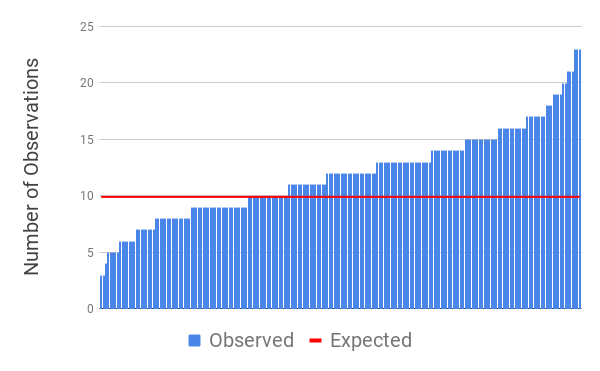
\includegraphics[width=.5\textwidth]{img/pairwiseL0Test.png}}}
	\subfloat[Unique Hash Map]{{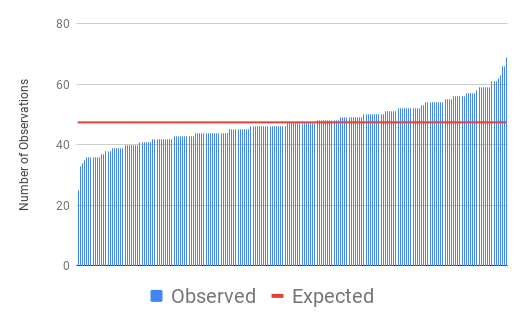
\includegraphics[width=.5\textwidth]{img/uniqueL0Test.png}}}
	\caption{Occurrences of each value in a sample when different hashing methods are used for $L_0$ sampling, order by increasing number of occurrences.}
	%"Final Evaluation - insertion-only"/Master
\end{figure}
%TODO map is now an array since vertices are zero-indexed and sequential (less space & quicker)
When implementing \texttt{$L_0$ Sampling} the main problem is how to implement the $k$-wise independent hash function efficiently. I looked into libraries which provided such functions but none allowed for the range to be controlled and taking the modulus with respect to $n^3$ breaks the independence property. Using a pairwise independent hash function would be ideal as they are easy to implement. \texttt{Figure 3.3.1 a)} shows the results when testing using a pairwise hash function. These results fail a $\chi^2$ test for a uniform distribution, indicating a pairwise independent hash function is not sufficient.

\par A \texttt{map} which assigns each value in $[n]$ to a distinct value in $[n^3]$, with values chosen uniformly at random, is equivalent to an $n$-wise independent hash function. The probability of a collision when assigning each value is less than $\frac1{n^2}$ meaning no collisions are expected when assigning values. This means that such a \texttt{map} is generated in $\mathcal{O}(n)$ time on average and requires $\mathcal{O}(n\log n)$ space. \texttt{Figure 3.3.1 b)} shows the results when such a \texttt{map} is implemented as the hash function $h$. These results pass a $\chi^2$ test for a uniform distribution so I implemented this \texttt{map} as the $k$-wise independent hash function. As the vertices are assumed to be labelled in $[n]$ this \texttt{map} can be implemented as an array with the hash values stored in each index. Using an array is more space-efficient than a tradition \texttt{map}.

\par The maximum hash value is a constraint on the size of the domain and thus the number of vertices which can be handled. In theory this is not a problem, but in practice the limit of this value depends on the data type used. I implemented the hash array as an array of \texttt{uint64\_t} (8 bytes) which has the greatest maximum value of the standard c++ numeric data type. The maximum domain is the cube root of this value, thus \textbf{Algorithm 8} will not work for graphs with more than $(2^{64}-1)^{1/3}\approx2.6\times10^6$ vertices and \textbf{Algorithm 9} will not work for graphs with more than $(2^{64}-1)^{1/6}\approx1,625$ vertices. This constraints can be reduced by reducing the relative range of the hash function.

\begin{figure}[H]
	\label{Figure 14}
	\subfloat[Varying $\delta$ ($\gamma=.1$)]{{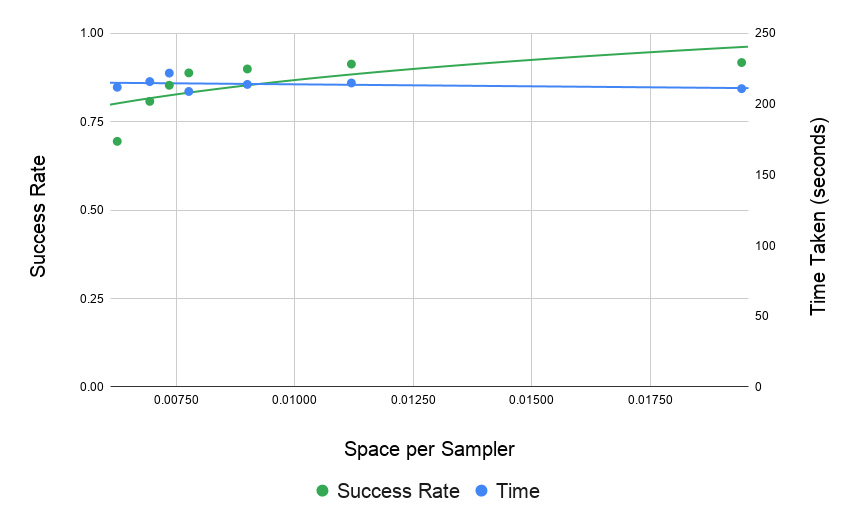
\includegraphics[width=.5\textwidth]{img/varyDelta.png}}}
	\subfloat[Varying $\gamma$ ($\delta=.2$)]{{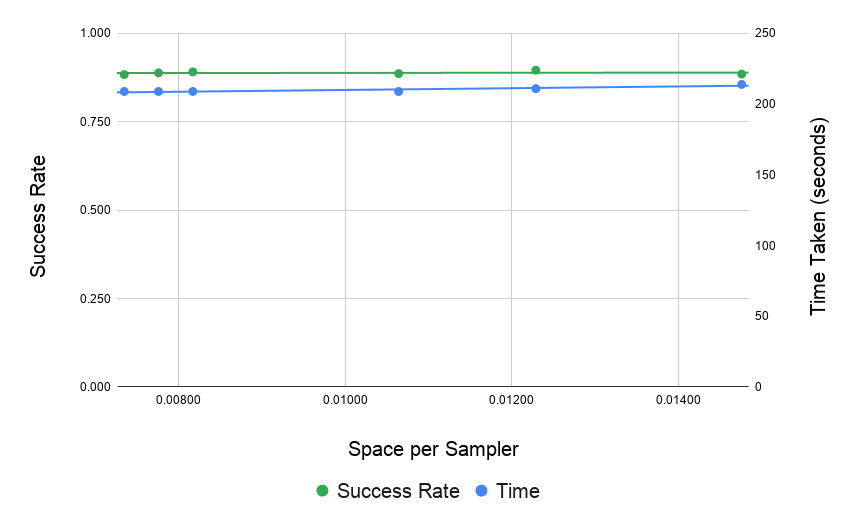
\includegraphics[width=.5\textwidth]{img/varyGamma.png}}}
	\caption{Space Usage and time taken when varying $\gamma$ and $\delta$ in $L_0$ Sampling implementation. For graph \texttt{facebook\_deletion}}
	%"Final Evaluation - insertion-only"/Master
\end{figure}

\par When setting $\gamma$ and $\delta$ there is a trade off between space-usage and the success rate. The value of $\delta$ affects the number of columns and rows in each $s$-sparse recovery, whereas $\gamma$ only affects the number of rows. Thus optimising $\delta$ first has the greatest effect. \texttt{Figure 3.3.2 a)} plots success-rate and time taken against space used when $\gamma=.1$ and $\delta$ is varied. The time taken is constant throughout, but the success rate plateaus at $\smallsim\!90\%$ when $d\geq.2$. \texttt{Figure 3.3.2 b)} shows that fixing $\delta=.2$ and varying $\gamma$ has no effect on performance. Thus $\gamma$ is set to .3 in order to minimise space usage.

\subsection{Vertex Sampling Algorithm} %TODO HERE
%\begin{itemize}
%	\item L0 samplers in parallel
%	\begin{itemize}
%		\item require lots of preallocated space (know how much space is used at start of algorithm)
%	\end{itemize}
%	\item Require list of vertices before vertex sampling.
%\end{itemize}

\par The vertex sample $A$ can be acquired by uniformly sampling from $[n]$ until a sufficient number of unique values is sampled. For a sample of size $m$, each time a vertex is sampled the probability of a collision is at most $\frac{m}n$ meaning the expected number of total collisions is at most $m$. Thus, in the worst case a sample is generated in $\mathcal{O}(mn)$ time.

\par The sampled edges form an insertion-only graph stream so a sufficient neighbourhood can be found among them using the algorithms discussed in \textbf{Chapter 2}. Due to the limitations from the $L_0$ sampler implementation I could not run this implementation on particular large graphs, this meant that the number of sampled edges is very small and thus the naive \textbf{Algorithm 4} provided the best results as it always succeeds. If the implementation was improved to run on larger graphs then \textbf{Algorithm 3} should be used for its overall performance improvements.

%\par Running $L_0$ samplers in parallel requires space being allocated for them before the stream is passed. This means all the space used by the algorithm (except that used to check for a sufficient neighbourhood) is known before the algorithm is run. This allows for a lot of evaluation of the space efficiency of the algorithm before implementation. %TODO consider removing

\begin{figure}[H]
	\label{Figure 15}
	\subfloat[Time Taken]{{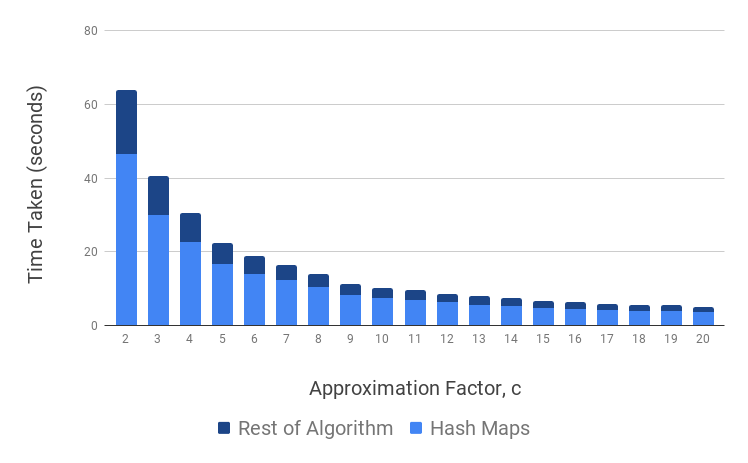
\includegraphics[width=.5\textwidth]{img/facebookDeletionInitialTime.png}}}
	\subfloat[Space Used]{{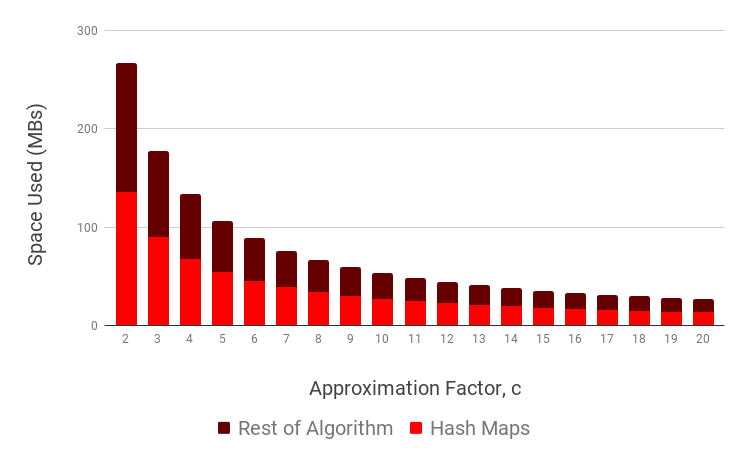
\includegraphics[width=.5\textwidth]{img/facebookDeletionInitialSpace.png}}}
	\caption{Space Usage and time taken for initial implementation of vertex sampling, for graph \texttt{facebook\_deletion}, when varying approximation factor.}
	%"insertion_deletion_facebook
\end{figure}

\texttt{Figure 3.3.3} shows the results of an initial implementation of vertex sampling. The proposed sample size would have been greater than $n$ for \texttt{facebook\_deletion} so $\sqrt{n}$ was used as a placeholder value until a more suitable sample size was tested for. This sample size proved too small for $c\leq4$ and resulted in some failures (Success rate remained above $83\%$ in all cases). These failures do not have a significant effect the performance of the algorithm as checking for sufficient neighbourhoods accounts for a small amount of the time and space usage. As expected, the hashing functions used in $L_0$ sampling account for the majority of space and time usage. Reducing the number of samplers will reduce the time and space usage of the implementation but will increase the failure rate if the number of unique edges sampled is reduced. The suggested number of samplers allows for a lot of redundancy as many edges are sampled multiple times.

\vspace{.3cm}\begin{adjustwidth}{.3cm}{}\fbox{\parbox{\textwidth}{

\textbf{Lemma 3.3} $\frac{\ln(1-p)}{\ln\left(1-\frac1m\right)}$ $L_0$ samplers are expected to find $p\delta$ unique neighbours of a vertex of degree $\delta$.\\

\textit{Proof} Consider a vertex $v$ of degree $\delta$ and let $i$ be a neighbour of $v$. Each $L_0$ sampler run on the edge vector of $v$ does not sample $i$ with probability $\frac{\delta-1}\delta$. As each sampler is independent the probability of $i$ not being sampled after $t$ $L_0$ samplers have been run is $\left(\frac{\delta-1}\delta\right)^t$. For the probability that $i$ has been sampled to be at least $p$ requires $\left(\frac{\delta-1}{\delta}\right)^t\leq 1-p$. This means $t\geq\frac{\ln(1-p)}{\ln\left(1-\frac1m\right)}$ samplers need to have been run. Since each neighbour is independent, $p$ is also the expected proportion of the neighbours which are sampled.

}}\end{adjustwidth}\vspace{.3cm}

\par \textbf{Lemma 3.3} tells us the minimum number of $L_0$ samplers required for us to expect a sufficient neighbourhood to a vertex to be found and by tuning the value of $p$ the number of samplers and achieved success rate can be optimised. When a vertex is sampled it is appropriate to assume it has at least degree $\frac{d}c$. The greater the actual degree of the vertex, the lower $p$ needs to be for $\frac{d}c$ neighbours to be returned as collisions are less likely. So tuning $p$ for vertices of degree close to $\frac{d}c$ is a good indicator of how vertices of greater degree will perform. Testing showed that setting $p=.9$ resulted in a sufficient neighbourhood being found $23\%$ of the time for a vertex of degree $\frac{11d}{10c}$ and $97\%$ of the time for a vertex of degree $\frac{12d}{10c}$. The implementation of $L_0$ samplers being used only successfully samples $90\%$ of the time, to account for this the expected number of samplers is multiplied by $\frac{1}{.9}$.

\begin{figure}[H]
	\label{Figure 16}
	\subfloat[Time Taken]{{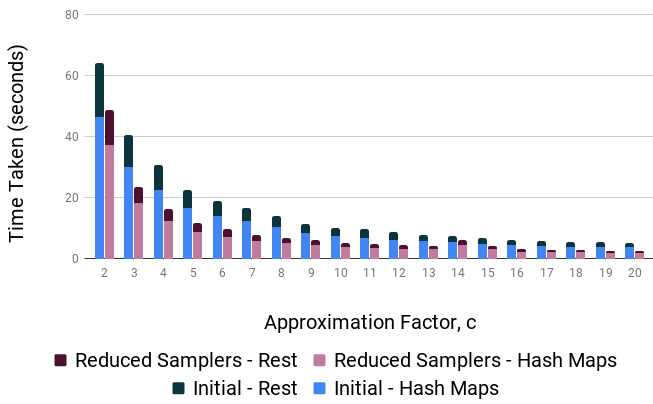
\includegraphics[width=.5\textwidth]{img/facebookDeletionSamplersPerVertexTime.png}}}
	\subfloat[Space Used]{{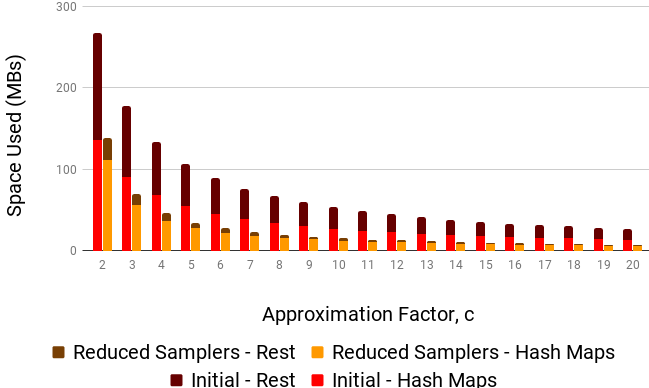
\includegraphics[width=.5\textwidth]{img/facebookDeletionSamplersPerVertexSpace.png}}}
	\caption{Time taken and space used when the number of $L_0$ samplers is optimised against the initial implementation, for graph \texttt{facebook\_deletion}, when varying approximation factor.}
	%"insertion_deletion_facebook"
\end{figure}
\texttt{Figure 3.3.4} shows the results when $\frac1{.9}\cdot\frac{\ln(1-.9)}{\ln(1-\frac{c}d)}$ samplers are run for each sampled vertex, rather than the suggested $10\frac{d}{c}\ln(n)$. The total space usage more than halved in all cases, and the space not used by the hash maps reduced by over $80\%$. The time taken by the algorithm (excluding that spent producing the hash maps) decreased by over $40\%$ in all cases. Both of these reductions are due to the total number of $L_0$ samplers being reduced. The success rate was unchanged, showing that there was a lot of redundancy in the number of samplers being run.

\par The optimal vertex sample size depends on the degree distribution of the graph as this describes how many vertices are of sufficient degree. Thus any prior knowledge of the degree distribution of the graph should be used. It is trivial to establish the degree distribution of a graph from a graph stream by counting the degree of each vertex although an exact distribution is not required as research has been done into typically degree distributions for common graphs from real world applications. In this project I have been using graphs from social networks which are theorised \cite{socialNetworkDistribution} to follow a Power-law distribution $f(x)=cx^{-\alpha}$. By Zipf's Law of Power-law distributions, the expected number of vertices of degree at least $\frac{d}{c}$ is $c$. Thus a uniform sample of $\frac{n}c$ vertices in $V$ is expected to contain a vertex of sufficient degree. A larger sample should be taken as it is not guaranteed that the maximum neighbourhood will be found for all sufficient vertices. Using this as a basis for the vertex sample size should make the algorithm very successful but as $\frac{n}c\gg\sqrt{n}$ for the most interesting values of $c$ its performance will be significantly worse.

\begin{figure}[H]
	\label{Figure 17}
	\subfloat[Time Taken]{{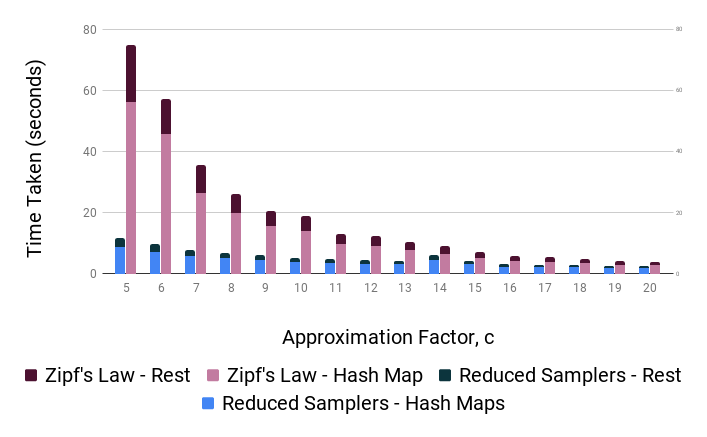
\includegraphics[width=.5\textwidth]{img/facebookDeletionVertexSampleSizeTime.png}}}
	\subfloat[Space Used]{{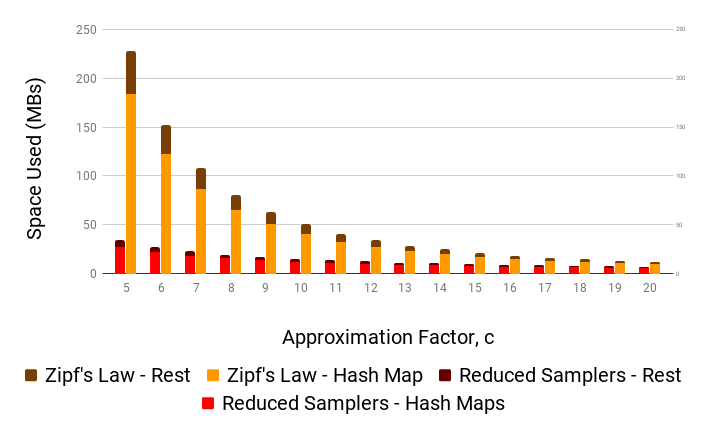
\includegraphics[width=.5\textwidth]{img/facebookDeletionVertexSampleSizeSpace.png}}}
	\caption{Space Usage and time taken when $\frac{12n}{10c}$ vertices are sampled against implementation of reduced number of sampelrs, for graph \texttt{facebook\_deletion}, when varying approximation factor.}
	%"Final Evaluation - insertion-only"/Master
\end{figure}

\texttt{Figure 3.3.5} shows the performance results when a vertex sample size of $\frac{12n}{10c}$ was taken compared to the initial $\sqrt{n}$. As predicted, the algorithm succeed in all cases where the new sample size was used however it's performance is significantly worse in all cases where $\frac{12n}{10c}\geq n$. The small size \texttt{facebook\_deletion} means that Zipf's Law is unlikely to fit well and it is theorised that the degree distribution of social networks have a fatter tail than a standard Power-law distribution. It is clear that further research is required into a performance optimal sample size for different scenarios.

\subsection{Edge Sampling Algorithm}

Running an $L_0$ sampler on the set of edges means the domain of the $k$-wise independent hash function is the edge set and thus we require a way of indexing the edges such that each has a unique value which can then be hashed. This indexing needs to be bijective so that the recovered index can be converted back into an edge. My initial implementation assigned the edge $(u,v)$ to $i=(\mathtt{min}(u,v)-1)\cdot n+\mathtt{max}(u,v)-1$ which maps edges to values in $[0,n^2)$. The use of \texttt{max} and min means that $(u,v)$ and $(v,u)$ map to the same value which is desirable since the edges are undirected. An edge can be recovered from this mapping as $\mathtt{min}(u,v)=(i\text{ mod }n)+1$ and $\mathtt{max}(u,v)=\mathtt{floor}(1/n)+1$. This mapping means the hash maps used in $L_0$ sampling now have $\mathcal{O}(n^2)$ space and time complexity. %TODO extracting edge from the key
\par As with the vertex sampling approach finding a sufficient neighbourhood in the sampled vertices should be done using the algorithms discussed in \textbf{Chapter 2}.

\begin{figure}[H]
	\label{Figure 18}
	\subfloat[Time Taken]{{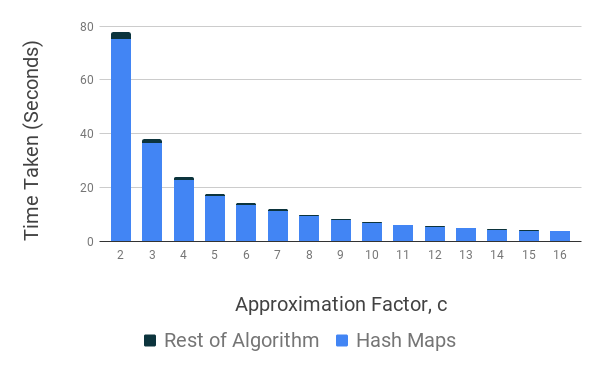
\includegraphics[width=.5\textwidth]{img/facebookSmallDeletionEdgeSampleSizeTime.png}}}
	\subfloat[Space Used]{{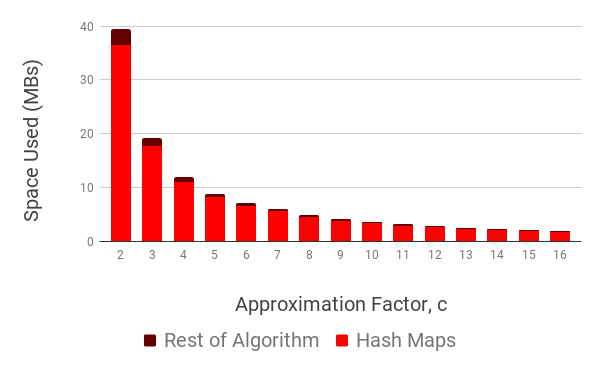
\includegraphics[width=.5\textwidth]{img/facebookSmallDeletionEdgeSampleSizeSpace.png}}}
	\caption{Space Usage and time taken for initial implementation of edge sampling, for graph \texttt{facebook\_small\_deletion}, when varying approximation factor.}
	%"Final Evaluation - insertion-only"/Master
\end{figure}

\texttt{Figure 3.3.6} shows the results from the initial implementation of \textbf{Algorithm 9}. As with the implementation of the vertex sampling algorithm, the majority of the space and time requirements are spent in generating the hash arrays for the $L_0$ samplers. The requirement for generating these is so high that I could not run the algorithm on \texttt{facebook\_deletion} as the space requirements were over $1$ GB and it took several minutes to generate a single hash array.

\begin{figure}[H]
	\label{Figure 19}
	\subfloat[Time Taken]{{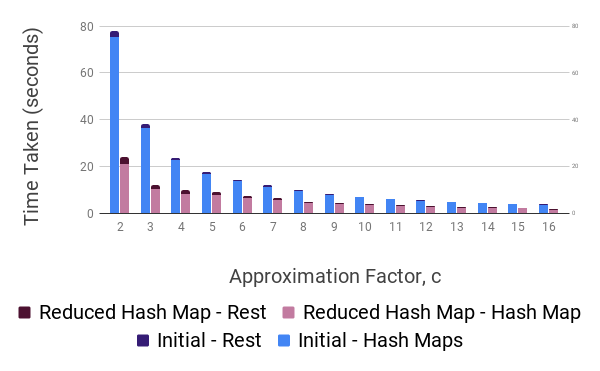
\includegraphics[width=.5\textwidth]{img/facebookSmallDeletionReducedHashMapTime.png}}}
	\subfloat[Space Used]{{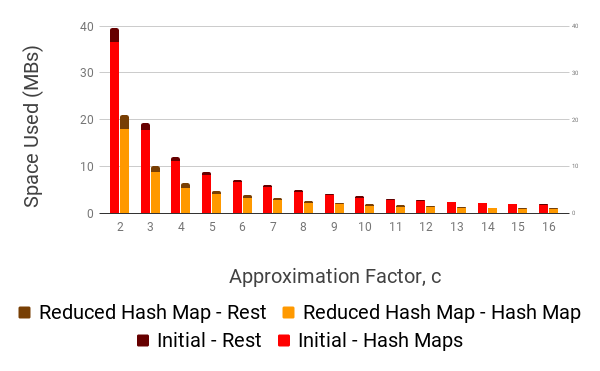
\includegraphics[width=.5\textwidth]{img/facebookSmallDeletionReducedHashMapSpace.png}}}
	\caption{Space Usage and time taken when a reduced hash map is implemented against the initial implementation of edge sampling, for graph \texttt{facebook\_small\_deletion}, when varying approximation factor.}
	%"Final Evaluation - insertion-only"/Master
\end{figure}

\par To reduce the size of the hash maps I changed how the edges were indexed. The graphs used in this project are undirected so have at most $\frac12n(n-1)$ unique edges. These can be visualised as the upper triangle of an adjacency matrix. The following formula map between an edge $(u,v)$ to key $k\in[\frac{1}{2}n(n-1)]$. In the implementation I ensured that $v>u$ so that the edges $(u,v)$ and $(v,u)$ mapped to the same $k$ and that the equations would succeed. % min & max
\[\begin{array}{rcl}
k&=&\frac12n(n-1)-\frac12(n-v)(n-v-1)+u+v-1\\
v&=&n-2-\text{floor}\left(\frac{1}2\sqrt{-8k+4n(n-1)-7}-\frac{1}2\right)\\
u&=&k+v+1-\frac12n(n-1)+\frac12(n-v)(n-v-1)
\end{array}\]
Implementing this method of indexing edges optimises the hash arrays but they still impact performance too much for the implementation to be usable on anything except the smallest of graphs.\texttt{Figure 3.3.7} shows the performance improvements from this implementation.

\par This implementation succeeded in every case due to large number of samplers successfully sampling every edge, this is inefficient as most of these edges went unused while checking for a sufficient neighbourhood. For larger graphs not all edges would be sampled as the relative difference between the number of edges and number of samplers decreases. However, this implementation is not usable on reasonably sized graphs so I cannot effectively test alterations to the number of samplers run. The edge sampling method should be designed to work in cases where the vertex sampling method fails. Primarily this is when it is unlikely that a sufficient vertex is sampled, this occurs in graphs where only a handful of vertices are of high degree and the rest are of very low degree. In these cases there are very few edges which do not involve a vertex of high degree and by estimating how many high degree vertices there are you can calculate the expected number of edges which need to be sampled before a sufficient neighbourhood is found.

\section{Evaluation}

The performance of the implementations of \textbf{Algorithm 8} and \textbf{Algorithm 9} are dominated by the hash functions used by the $L_0$ samplers. This meant that the implementations could not be run on graphs of sufficient size to evaluate certain aspects of the implementations, namely the vertex sample size in \textbf{Algorithm 8} and number of samples in \textbf{Algorithm 9}. As well, it would be inappropriate to compare the performance to that of the naïve algorithm described in \textbf{Algorithm 11} as the proposed algorithms account for very little of the time and space of the whole implementation.

\begin{algorithm}[H]
\caption{Na\"ive Single-Pass Insertion-Streaming Algorithm for Neighbourhood Detection}
\SetKwInOut{Require}{require}
\Require{Stream $\{(w_0,s_0,t_0)\dots(w_n,s_n,t_n)\}$, degree bound $d$, precision bound $c$}
$N\leftarrow\{\{\}\}\ \{\text{neighbourhoods}\}$\\
\For{$i=0\dots n$} {
	\lIf{$w_i\equiv1$}{append $t_i$ to $N[s_i]$\hfill \texttt{// Insertion instruction}}
	\lElseIf{$w_i\equiv-1$}{remove $t_i$ from $N[s_i]$\hfill \texttt{// Deletion instruction}}
}
\tcp{Look for a sufficiently large neighbourhood}
\For{$s_i\in N.keys$}{
	\If{\text{size}($N[s_i])\geq d$} {
		\tcp{Sufficiently large neighbourhood found}
		$S\leftarrow \{N[s_i][0],\dots,N[s_i][\frac{d}{c}]\}$\tcp*{First $\frac{d}c$ elements of neighbourhood}
		\Return{($s_i,S$)}
	}
}
\Return{FAIL\hfill\texttt{No sufficient neighbourhoods}}
\end{algorithm}

\par I will briefly discuss the na\"ive algorithm as it may be useful for future projects. \textbf{Algorithm 11} is very similar to the na\"ive implementaiton given for insertion-only streams \textbf{Algorithm 4} in that it records the neighbourhood for every vertex. However, it does not have the efficiency of terminating after find the first sufficient neighbourhood as it is possible for that neighbourhood to shrink later in the stream. This method will see no significant variation in performance when $c$ is varied as it will produce the same set of neighbourhoods in every case. This method uses $\mathcal{O}(n^2)$ space for all values of $c$.

\chapter{Conclusions}

\section{Achievements}

The algorithm proposed in \cite{orig} for insertion-only graphs proves very practical for solving \texttt{neighbourhood detection} on real world graphs. The changes to the implementations made reduced the time and space used by the algorithm significantly, while not compromising on the success rate. The final evaluation shows that the proposed algorithm is much more space-efficient than a naïve approach. Even for close approximations of large streams the final implementation uses less than $6\%$ of the file size and for $c\geq5$ it uses $\leq1\%$. This space efficiency increases the maximum file size at which the algorithm is usable, without requiring virtual memory. The run-times of my final implementation are very usable with solutions being found for a graph of over 30 million edges in a couple of minutes for close approximations $c\in[2,4]$.
\par My main contribution to the proposed insertion-deletion algorithm is the demonstration of how limiting a poor implementation of $k$-wise independent hash family is to the practicalities of this algorithm. Research into possible implementations of these hashing families would consistute a significant and useful future project.
\par Due to the difficulties in generating functions from a $k$-wise independent hashing family the proposed algorithm for insertion-deletion graphs could not be evaluated on graphs which were sufficiently large as to be interesting. However, I still managed to discuss several improvements to the implementation. The simplification of \texttt{1-sparse recovery} to only require two counters is a great improvement as, when the hash function is discounted, the \texttt{1-sparse recoveries} account for the majority of the space used by the $L_0$ samplers and thus both proposed algorithms. The probabilistic approach taken to reduce the number of $L_0$ samplers run for each vertex significantly improved performance by reducing redundancy, without compromising success. The indexing method which mapped edges to unique values in $\left[0,\frac12n(n-1)\right)$ was a really good improvement as it is the optimal indexing method for undirected graphs.

\section{Future Work}

To conclude this project I will mention a few areas that I think any further evaluation of the algorithms proposed in \cite{orig} should consider.

\subsection*{Complete Real World Evaluation}
In this project I soley used graphs from social networks as they were readily available and an area where \texttt{neighbourhood detection} is an interesting problem. It would be interesting to test the implementations produced in this project on data sets from other fields. Section \texttt{I.ii Motivating Applications} provides a few examples. Further, it would be interesting to investigate how the returned neighbourhood is used to draw inferences about the graph as this would provide greater direction to how the implementations should be optimised. A possible problem could be detecting DDOS attacks from a network log.

\subsection*{$k$-Wise Independent Hashing Family}
An alternative family of $k$-wise independent hash function is ${\displaystyle h(x)=\left(\left(\sum_{i=0}^{k-1}a_ix^i\right)\text{mod }P\right)\text{mod }m}$ where $a_0>0$ and $a_i<P\ \forall\ i$. A function from this family is quick to generate as only the $k$ $a_i$ values need to be random generated and can be stored as $k+2$ integers (the values of $a_i$, $k$ and $m$). Both of these are dramatic improvements from the implementation of hash arrays used in the implementation of an $L_0$ sampler. The difficulty with implementation functions from this family is that the values of $x^i$ quickly overflow causing inaccurate calculations. I am sure an implementation of this family of hash functions could be worked out, but I ran out of time to do so in this project.

\subsection*{Vertex Sample Size}
I discussed how the size of the vertex sample used in \textbf{Algorithm 8} should depend on the degree distribution of the graph, and investigated one line of thought for how this could be done for graphs of social network connections. Investigating this further was outside the scope of this project but would be an interesting feature to research further.
\par The edge sampling approach proposed in \textbf{Algorithm 9} should be considered whilst evaluating the size of the vertex sample, as there will be cases where this approach is more efficient. The most obvious example of this would be a star graph where the vertex sampling approach would need to sample every vertex in order to guarantee find a sufficient neighbourhood, whereas the edge sampling approach only needs to sample $\frac{d}c$ edges. In more general scenarios it is likely that the edge sampling approach is better for close approximations and the vertex sampling approach better for loser approximations.

\subsection*{Reservoir Sample Size}
I tested changing the reservoir sample size used in \textbf{Algorithm 2} but no strategies where found which consistently improved performance. These tests changed the sample size of every sampler used, but it may be that reducing the sample size for later samplers produces good results as those samplers are sampling for a smaller pool. This would be the main feature to look at when further trying to optimised the implementation from \textbf{Chapter 2}.

\begin{thebibliography}{4}
	\addcontentsline{toc}{chapter}{Bibliography}
	\bibitem{orig} Christian Konrad \textit{Streaming Frequent Items with Timestamps and Detecting Large Neighborhoods in Graph Streams.} November 2019.
	\bibitem{SNAP}http://snap.stanford.edu/data/
	\bibitem{L0Framework} Graham Cormode, Donatella Firmani \textit{A Unifying Frameworkd for $\ell_0$-Sampling Algorithms.} September 2014.
  \bibitem{socialNetworkDistribution} Tushti Rastogi \textit{A power law approach to estimating fake social network accounts.} May 2016.
  \bibitem{GraphStreamSurvey} Andrew McGregor \textit{Graph Stream Algorithms: A Survey.} May 2014.
  \bibitem{clusteringCofficient} Madhav Jha, C. Seshadhri, and Ali Pinar \textit{A space-efficient streaming algorithm for estimating transitivity and triangle counts using the birthday paradox.} February 2015.
  \bibitem{edgesOfSpanner} B\'ela Bollob\'as \textit{Extremal Graph Theory.} 1978
  \bibitem{spanner} Surender Baswana \textit{Streaming Algorithm for Graph Spanners - Single Pass and Constant Processing Time per Edge.} April 2008.
  \bibitem{RandomWalks} Atish Das Sarma, Sreenivas Gollapudi, and Rina Panigraphy \textit{Estimating PageRank on Graph Streams.} May 2011.
  \bibitem{degResSampling} Jeffery Vitter \textit{Random Sampling with a Reservoir.} Match 1985.
\end{thebibliography}

\end{document}
